%%%%%%%%%%%%%%%%%%%%%%%%%%%%%%%%%%%%%%%%%%%%%%%%%%%%%%%%%%%%%%%%%%%%%%%%%%%%%%%%
%% Plantilla de memoria en LaTeX para TFG/TFM - Universidad Rey Juan Carlos
%%
%% MEMORIA PROYECTO - TFG Cristina Gallego Herrero
%%
%% Por Gregorio Robles <grex arroba gsyc.urjc.es>
%%     Felipe Ortega   <felipe.ortega@urjc.es>
%%     Grupo de Sistemas y Comunicaciones (GSyC)
%%     Escuela Técnica Superior de Ingenieros de Telecomunicación
%%     Universidad Rey Juan Carlos
%%
%% (Muchas ideas tomadas de Internet, colegas del GSyC, antiguos alumnos...
%%  etc. Muchas gracias a todos)
%%
%% La última versión de esta plantilla está siempre disponible en:
%%     https://github.com/glimmerphoenix/plantilla-memoria
%%
%% - Ejecución en sistema local:
%% Para obtener el documento en PDF, ejecuta en la shell:
%%   make
%%
%% A diferencia de la anterior versión, que usaba la herramienta pdfLaTeX 
%% para compilar el documento, esta nueva versión de la plantilla usa
%% XeLaTeX. Es un compilador más moderno que, entre otras mejoras, incluye
%% soporte nativo para caracteres con codificación UTF-8, traducción políglota
%% de referencias (usando Biblatex) y soporte para fuentes OTF. Esta última
%% característic permite, por ejemplo, insertar iconos de la colección 
%% Fontawesome en el texto.
%%
%% XeLaTeX viene ya incluido en todas las distribuciones modernas de LaTeX.
%%
%% - Edición y ejecución en línea: 
%% Puedes descargar y subir la plantilla a
%% Overleaf, un editor de LaTeX colaborativo en línea. Overleaf ya tiene
%% instalados todos los paquetes LaTeX y otras dependencias software para
%% que esta plantilla compile correctamente.
%%
%% IMPORTANTE: Si compilas este documento en Overleaf, recuerda cambiar
%% la configuración (botón "Menu" en la esquina superior izquierda de la interfaz)
%% y elegir la opción Compiler --> XeLaTeX. En caso contrario no funcionará.
%%
%% - Nota: las imágenes deben ir en PNG, JPG, EPS o PDF. También se pueden usar
%% imágenes en otros formatos con algunos cambios en el preámbulo del documento.

%%%%%%%%%%%%%%%%%%%%%%%%%%%%%%%%%%%%%%%%%%%%%%%%%%%%%%%%%%%%%%%%%%%%%%%%%%%%%%%%

\documentclass[a4paper, 12pt]{book}

%%-- Geometría principal (dejar activada la siguiente línea en la versión final)
\usepackage[a4paper, left=2.5cm, right=2.5cm, top=3cm, bottom=3cm]{geometry}
%%-- Activar esta línea y comentar la anterior en modo borrador, para comentarios al margen
%\usepackage[a4paper, left=2.5cm, right=2.5cm, top=3cm, bottom=3cm, marginparwidth=60pt]{geometry}

%%-- Hay que cargarlo antes que las traducciones
\usepackage{listing}                    % Listados de código

% Traducciones en XeLaTeX
\usepackage{polyglossia}
\setmainlanguage{spanish}    % Comenta esta línea si tu memoria es en inglés

% Traducciones particulares para español
% Caption tablas
\gappto\captionsspanish{
	\def\tablename{Tabla}
	\def\listingscaption{Código}
	\def\refname{Bibliografía}
	\def\appendixname{Apéndice}
	\def\listtablename{Índice de tablas}
	\def\listingname{Código}
	\def\listlistingname{Índice de fragmentos de código}
}

%% Tipografía y estilos
\usepackage[OT1]{fontenc}               % Keeps eulervm happy about accents encoding

% Símbolos y fuentes matemáticas elegantes: Euler virtual math fonts
% ¡Importante! Carga siempre las fuentes math AMS Euler ANTES QUE fontspec
\usepackage{amsmath}
\usepackage{amssymb}
\usepackage[OT1,euler-digits,euler-hat-accent,small]{eulervm}

% En XeLaTeX las fuentes se especifican con fontspec
\usepackage{fontspec}
\defaultfontfeatures{Scale=MatchLowercase, Ligatures=TeX}     % Default option in font config

% Fix para fuentes usadas con operadores y \mathrm
\DeclareSymbolFont{operators}{\encodingdefault}{\familydefault}{m}{n}

% Configura la fuente principal (serif): MinionPro
\setmainfont[Scale=0.96]{TeX Gyre Pagella}
% Configura la fuente sans-serif (\sffamily)
\setsansfont[Scale=MatchLowercase]{Lato}
% Configura la fuente para letra monoespaciada: Source Code Pro, escala 0.85
\setmonofont[Scale=0.85]{Source Code Pro}

%%-- Familias de fuentes específicas
%%-- Se pueden definir etiquetas para familias de fuentes personalizadas
%%-- que luego puedes emplear para cambiar el formato de una parte de texto
%%-- Ejemplo:
% \newfontfamily{\myriadprocond}{Myriad Pro Semibold Condensed.otf}

%%-- Opciones de interlineado y espacios
\linespread{1.07}                   % Aumentar interlineado para fuentes tipo Palatino
\setlength{\parskip}{\baselineskip} % Separar párrafos con línea en blanco

%%-- Hipervínculos
\usepackage{url}

%%-- Gráficos y tablas
\PassOptionsToPackage{
    dvipdfmx,usenames,dvipsnames,
    x11names,table}{xcolor}             % Definiciones de colores
\PassOptionsToPackage{xetex}{graphicx}

\usepackage{subfig}                     % Subfiguras
\usepackage{pgf}
\usepackage{svg}                        % Integración de imágenes en formato SVG
\usepackage{float}                      % H para posicionar figuras
\usepackage{booktabs}                   % Already loads package xcolor
\usepackage{multicol}                   % multiple column layout facilities
\usepackage{colortbl}                   % For coloured tables
\usepackage{wrapfig}                    % Envolver texto en las figuras
\usepackage{capt-of}
\usepackage{multirow}                   % Multirow tablas
%%-- Bibliografía con Biblatex y Biber
% Más info:
% https://www.overleaf.com/learn/latex/Biblatex_bibliography_styles
% https://www.overleaf.com/learn/latex/biblatex_citation_styles
\usepackage[
    backend=biber,
    style=numeric,
    sorting=none
    ]{biblatex}
\addbibresource{refs.bib}
\DeclareFieldFormat{url}{\mkbibacro{URL}\addcolon\nobreakspace\url{#1}}
%\usepackage[nottoc, notlot, notlof, notindex]{tocbibind} %% Opciones de índice

%%-- Matemáticas e ingeniería
% El paquete units permite mostrar unidades correctamente
% Permite escribir unidades con espaciado y estilo de fuente correctos
\usepackage[ugly]{units}         
% Ejemplo de uso: $\unit[100]{m}$ or $\unitfrac[100]{m}{s}$
% Entornos matemáticos
\newtheorem{theorem}{Theorem}

% Paquetes adicionales
\usepackage{url}                        %% Gestión correcta de enlaces
\usepackage{float}                      %% H para posicionar figuras
\usepackage[nottoc, notlot, notlof, notindex]{tocbibind}    %% Opciones de índice
\usepackage{metalogo}                   %% Múltiples logos para XeLaTeX

% Fuentes especiales y glifos
\usepackage{ccicons}                % Creative Commons icons
\usepackage{metalogo}               % XeTeX logo
\usepackage{fontawesome5}           % Fontawesome 5 icons
\usepackage{adforn} 

% Blindtext
% Opciones pangram, bible, random (defecto)
\usepackage[pangram]{blindtext}
% Lorem ipsum
\usepackage{lipsum}
% Kant lipsum
\usepackage{kantlipsum}

\usepackage{fancyvrb}               % Entornos verbatim extendidos
	\fvset{fontsize=\normalsize}    % Tamaño de fuente por defecto en fancy-verbatim
	
% Configura listas (itemize, enumerate) con iconos personalizados
% Fácil reinicio de numeración con enumerate
% Info: http://ctan.org/pkg/enumitem
\usepackage[shortlabels]{enumitem}
% Usar \usageitem para configurar iconos personalizados en listas
\newcommand{\usageitem}[1]{%
	\item[%
	{\makebox[2em]{\strut\color{GSyCblue} #1}}%
	]
}

%%-- Definición de colores personalizados
% \definecolor{LightGrey}{HTML}{EEEEEE}
% \definecolor{darkred}{rgb}{0.5,0,0}     %% Refs. cruzadas
% \definecolor{darkgreen}{rgb}{0,0.5,0}   %% Citas bibliográficas
% \definecolor{darkblue}{rgb}{0,0,0.5}    %% Hiperenlaces ordinarios (también ToC)

%%-- Configuración fragmentos de código
%%-- Minted necesita Python Pygments instalado en el sistema para funcionar

\usepackage{minted}

%%-- Se debe cargar aquí para evitar warnings
\usepackage{csquotes}                   % Para traducciones con biblatex

%%-- Glosario de términos
\usepackage[acronym]{glossaries}
\makeglossaries
\loadglsentries{glossary}

% % Definición de cabeceras del documento, usando fancyhdr
% \usepackage{fancyhdr}
% %% Configuración de cabeceras para el cuerpo principal del documento
% \pagestyle{fancy}
% \fancyhead{}
% \fancyhead[RO,LE]{\myriadprocond{\thepage}}
% \renewcommand{\chaptermark}[1]{\markboth{\chaptername\ \thechapter.\ #1}{}}
% \renewcommand{\sectionmark}[1]{\markright{\thesection.\ #1}}
% \fancyhead[RE]{\myriadprocond{\leftmark}}
% \fancyhead[LO]{\myriadprocond{\rightmark}}
% \renewcommand{\headrulewidth}{0pt}
% \setlength{\headheight}{15pt} %% Al menos 15pt para evitar warning al compilar
% \fancyfoot{}
% %% Configuración para páginas con cabecera en blanco
% \fancypagestyle{plain}{%
% \fancyhf{}% clear all header and footer fields
% \fancyhead[RO,LE]{\myriadprocond{\thepage}}
% \renewcommand{\headrulewidth}{0pt}%
% \renewcommand{\footrulewidth}{0pt}%
% }

%%-- Metadatos del doc
\title{Memoria del Proyecto}
\author{Nombre del autor}

%%-- Hiperenlaces, siempre se carga al final del preámbulo
\usepackage[colorlinks]{hyperref}
\hypersetup{
    pdftoolbar=true,	% Muestra barra de herramientas en Adobe Acrobat
	pdfmenubar=true,	% Muestra menú en Adobe Acrobat
	pdftitle={Título doc en ventana del visor o navegador},
	pdfauthor={Nombre del alumno/a},
	pdfcreator={ETSII/ETSIT, URJC},
	pdfproducer={XeLaTeX},
	pdfsubject={Topic1, Topic2, Topic3},
	pdfnewwindow=true,              %links open in new window
    colorlinks=true,                % false: boxed links; true: coloured links
    linkcolor=Firebrick4,           % enlaces internos 
    citecolor=Aquamarine4,          % enlaces a citas bibliográficas
    urlcolor=RoyalBlue3,            % hiperenlances ordinarios
    linktocpage=true                % Enlaces en núm. pág. en ToC
}

%%%---------------------------------------------------------------------------
% Comentarios en línea de revisión
% Este bloque se puede borrar cuando finalizamos el borrador

% \usepackage[colorinlistoftodos]{todonotes}
% \usepackage{verbatim}
%%%---------------------------------------------------------------------------

\begin{document}

%%-- Configuración común para todos los entornos listing
%%-- Descomentar para usar y personalizar valores
%\lstset{%
%breakatwhitespace=true,
% breaklines=true, 
% basicstyle=\footnotesize\ttfamily,
% keywordstyle=\color{blue},
% commentstyle=\color{green!40!black}, 
% language=Python} 
 

%%%%%%%%%%%%%%%%%%%%%%%%%%%%%%%%%%%%%%%%%%%%%%%%%%%%%%%%%%%%%%%%%%%%%%%%%%%%%%%%
% PORTADA

\begin{titlepage}
\begin{center}
\begin{tabular}[c]{c c}
%\includegraphics[bb=0 0 194 352, scale=0.25]{logo} &
\includegraphics[scale=1.5]{img/LogoURJC.png}
%&
%\begin{tabular}[b]{l}
%\Huge
%\textsf{UNIVERSIDAD} \\
%\Huge
%\textsf{REY JUAN CARLOS} \\
%\end{tabular}
\\
\end{tabular}

\vspace{3cm}

\Large 
INGENIERÍA EN TECNOLOGÍAS DE LA TELECOMUNICACIÓN 

\vspace{0.4cm}

\large
Curso Académico 2021/2022

\vspace{0.8cm}

Trabajo Fin de Grado

\vspace{2cm}

\LARGE HERRAMIENTAS PARA ANÁLISIS Y VISUALIZACIÓN \\
DE LA EVOLUCIÓN DE COMUNIDADES ONLINE DE PREGUNTA-RESPUESTA 
\vspace{3cm}

\large
Autora : María Cristina Gallego Herrero \\
Tutor : Dr. Felipe Ortega 
\end{center}
\end{titlepage}

\newpage
\mbox{}
\thispagestyle{empty} % para que no se numere esta pagina


%%%%%%%%%%%%%%%%%%%%%%%%%%%%%%%%%%%%%%%%%%%%%%%%%%%%%%%%%%%%%%%%%%%%%%%%%%%%%%%%
%%%% Para firmar
\clearpage
\pagenumbering{gobble}
\chapter*{}

\vspace{-4cm}
\begin{center}
\LARGE
\textbf{Trabajo Fin de Grado/Máster}

\vspace{1cm}
\large
Herramientas para Análisis y Visualización de la Evolución de Comunidades Online de Pregunta-Respuesta

\vspace{1cm}
\large
\textbf{Autora :} María Cristina Gallego Herrero  \\
\textbf{Tutor :} Dr. Felipe Ortega 

\end{center}

\vspace{1cm}
La defensa del presente Proyecto Fin de Grado se realiza el día \qquad$\;\,$ de
\qquad\qquad\qquad\qquad \newline de 20XX, siendo calificada por el siguiente tribunal:


\vspace{0.5cm}
\textbf{Presidente:}

\vspace{0.8cm}
\textbf{Secretario:}

\vspace{0.8cm}
\textbf{Vocal:}


\vspace{0.8cm}
y habiendo obtenido la siguiente calificación:

\vspace{0.8cm}
\textbf{Calificación:}


\vspace{0.8cm}
\begin{flushright}
Móstoles/Fuenlabrada, a \qquad$\;\,$ de \qquad\qquad\qquad\qquad de 20XX
\end{flushright}

%%%%%%%%%%%%%%%%%%%%%%%%%%%%%%%%%%%%%%%%%%%%%%%%%%%%%%%%%%%%%%%%%%%%%%%%%%%%%%%%
%%%% Dedicatoria

\chapter*{}
%\pagenumbering{Roman} % para comenzar la numeración de paginas en numeros romanos
\begin{flushright}
\textit{Dedicado a mi familia \\
y amigos.}
\end{flushright}

%%%%%%%%%%%%%%%%%%%%%%%%%%%%%%%%%%%%%%%%%%%%%%%%%%%%%%%%%%%%%%%%%%%%%%%%%%%%%%%%
%%%% Agradecimientos

\chapter*{Agradecimientos}
%\addcontentsline{toc}{chapter}{Agradecimientos} % si queremos que aparezca en el índice
\markboth{AGRADECIMIENTOS}{AGRADECIMIENTOS} % encabezado 

En primer lugar quiero agradecérselo a mi familia. A mis padres, pues sin ellos y sin su esfuerzo no hubiese sido capaz de cerrar este ciclo. Vosotros habéis sido el consuelo y el apoyo que necesitaba en los momentos más duros. Sin duda agradecer a mi hermano, Miguel, y a Tania, muchos han sido los días que habéis estado a mi lado, aguantando mis nervios y mis miedos. Sois y seréis mi mejor ejemplo a seguir, gracias.

Gracias a mis amigas, mis niñas desde que teníamos 3 años. Hemos crecido, vivido los mejores y peores momentos y, sobre todo, disfrutado cada etapa de nuestras vidas. No puedo ser más afortunada teniéndoos.

A mi pareja, mi compañero de vida. Gracias por tu paciencia y apoyo. No podría haber elegido mejor. 

Por último, quiero agradecer a mi tutor, Felipe, por darme ánimos para terminar el \acrshort{tfg}. Pero, sobre todo, gracias por ser paciente, por entender y comprender mi situación durante estos años.

A todos, gracias.

%%%%%%%%%%%%%%%%%%%%%%%%%%%%%%%%%%%%%%%%%%%%%%%%%%%%%%%%%%%%%%%%%%%%%%%%%%%%%%%%
%%%% Resumen

\chapter*{Resumen}
%\addcontentsline{toc}{chapter}{Resumen} % si queremos que aparezca en el índice
\markboth{RESUMEN}{RESUMEN} % encabezado

Hoy en día, la mayor parte de las aplicaciones y sistemas de comunicación presentan, trasfieren y almacenan grandes cantidades de información en tiempo real y son guardadas para su análisis tanto presente como futuro. 
Para poder dar un uso eficiente es necesario almacenar estos datos de manera ordenada y, si es posible, procesarlos de manera sencilla, visual e intuitiva.

Este análisis permite detectar errores, observar y analizar las variaciones en el tiempo y poder obtener análisis estadísticos o, incluso, realizar predicciones de  comportamiento. 

Este Trabajo de Fin de Grado consiste en la recopilación y análisis de datos mediante el uso de varias tecnologías de exploración y administración de datos. En este proyecto, se ha trabajado con Stack Exchange, que una red de webs de preguntas y respuestas sobre distintos temas. Contiene la información de Stack Overflow y otras comunidades similares. Estos datos se extraen y se almacenan en una base de datos para, posteriormente, visualizarlos en las herramientas gráficas que vamos a comparar durante el proyecto y sacar conclusiones dependiendo de diferentes criterios de comparación.

Hemos decidido centrarnos en dos herramientas principales: Grafana para análisis y visualización de los datos y Tableau, que realiza tanto el preprocesado de datos, el análisis y la visualización.

%%%%%%%%%%%%%%%%%%%%%%%%%%%%%%%%%%%%%%%%%%%%%%%%%%%%%%%%%%%%%%%%%%%%%%%%%%%%%%%%
%%%% Resumen en inglés

\chapter*{Summary}
%\addcontentsline{toc}{chapter}{Summary} % si queremos que aparezca en el índice
\markboth{SUMMARY}{SUMMARY} % encabezado

Nowadays, most applications and communication systems transfer and store large amounts of data in real-time and are stored for present and future analysis. 
In order to make efficient use of these data, that is necessary to store them in an orderly manner and process them in a simple, visual and intuitive way.

This allows you to detect errors, observe and analyze variations over time and to obtain statistical analysis or to make predictions about the behaviour of the system.

This Final Degree Project consists basically of the collection and analysis of data through the use of various technologies for data exploration and management. We have worked with Stack Exchange, a network of question-and-answer websites like Stack Overflow and other similar communities. This data is stored on a database, and later visualized in the graphical tools, we are going to compare during the project and to draw conclusions depending on different benchmarks.

We have decided to focus on two main tools. Grafana for data analysis and visualization and, on the other, Tableau to clean, analyze and visualize data.


%%%%--------------------------------------------------------------------
% Lista de comentarios de revisión
% Se puede borrar este bloque al acabar el borrador

%\listoftodos
%\markboth{TODO LIST}{TODO LIST} % encabezado
%%%%--------------------------------------------------------------------

%%%%%%%%%%%%%%%%%%%%%%%%%%%%%%%%%%%%%%%%%%%%%%%%%%%%%%%%%%%%%%%%%%%%%%%%%%%%%%%%
%%%%%%%%%%%%%%%%%%%%%%%%%%%%%%%%%%%%%%%%%%%%%%%%%%%%%%%%%%%%%%%%%%%%%%%%%%%%%%%%
% ÍNDICES %
%%%%%%%%%%%%%%%%%%%%%%%%%%%%%%%%%%%%%%%%%%%%%%%%%%%%%%%%%%%%%%%%%%%%%%%%%%%%%%%%

% Las buenas noticias es que los índices se generan automáticamente.
% Lo único que tienes que hacer es elegir cuáles quieren que se generen,
% y comentar/descomentar esa instrucción de LaTeX.

%%-- Índice de contenidos
\tableofcontents 
\cleardoublepage
%%-- Índice de figuras
%\addcontentsline{toc}{chapter}{Lista de figuras} % para que aparezca en el índice de contenidos
\listoffigures % indice de figuras
\cleardoublepage
%%-- Índice de tablas
%\addcontentsline{toc}{chapter}{Lista de tablas} % para que aparezca en el índice de contenidos
\listoftables % indice de tablas
\cleardoublepage
%%-- Índice de fragmentos de código
\listoflistings

%%%%%%%%%%%%%%%%%%%%%%%%%%%%%%%%%%%%%%%%%%%%%%%%%%%%%%%%%%%%%%%%%%%%%%%%%%%%%%%%
%%%%%%%%%%%%%%%%%%%%%%%%%%%%%%%%%%%%%%%%%%%%%%%%%%%%%%%%%%%%%%%%%%%%%%%%%%%%%%%%
% INTRODUCCIÓN %
%%%%%%%%%%%%%%%%%%%%%%%%%%%%%%%%%%%%%%%%%%%%%%%%%%%%%%%%%%%%%%%%%%%%%%%%%%%%%%%%

\cleardoublepage
\chapter{Introducción}
\label{sec:intro}
\pagenumbering{arabic} % para empezar la numeración de página con números
La información es poder,\textit{“Scientia potentia est”}:
el conocimiento es poder, decía Thomas Hobbes  en el \textit{Leviatán (1688)}. Hoy en día, vivimos en un mundo en constante revolución tecnológica, almacenamos todo tipo de información en bases de datos, y estas bases necesitan de técnicas y herramientas de análisis para obtener la mayor eficiencia.
Todo el conjunto de datos , procesos y análisis se denomina Big Data~\cite{mayer2013big}.

El análisis de datos trata de obtener conclusiones significativas sobre los datos que se analizan. Para ello se aplican técnicas estadísticas y lógicas, modulación de la estructura de los datos y la representación de estos mediante imágenes, tablas y gráficos~\cite{aranda2009tecnicas}.
%% Es *** increíble lo que se usa en todos los ámbitos ***
%%Antes de comenzar con el análisis de los datos, existe una etapa que trata de identificar y clasificar. Este proceso consiste en definir el alcance para tomar las especificaciones de los requisitos de los datos, su recolección  y procesamiento. Se necesita identificar los datos relevantes para su análisis y derivar una conclusión precisa.\newline 
Los siguientes pasos ayudan a identificar y clasificar los datos para su análisis: 
 \begin{itemize}
        \item Definición y especificación de los requisitos de los datos: Definir el alcance, los parámetros, unidades de medida\ldots
        \item Recolección de datos: Recopilación de los datos de la fuente.
        \item Procesamiento de datos: Organizar y estructurar los datos.
        \item Análisis de datos: Manipular y organizar los datos para visualizarlos.
        \item Interpretación de los resultados.
    \end{itemize}

En este proyecto se realizan los pasos anteriormente indicados, centrándonos en el análisis e interpretación de los resultados mostrados mediante dos herramientas software. Además, se compararán en base a diferentes criterios de comparación como es su usabilidad, uso principal, visualización, tamaño de las muestras y costes. 


\section{Planteamiento del problema}
\label{sec:seccion}

Hoy en día la visualización de la información tiene un valor muy importante, ya que es una manera sencilla de llegar a todos los públicos. Actualmente, todas las empresas de cualquier ámbito utilizan alguna herramienta de análisis que les permita visualizar y analizar los datos de manera centralizada. 

Existen múltiples herramientas que permiten esta visualización y análisis, durante este proyecto, se realiza la comparación basándonos en diferentes criterios de dos herramientas que actualmente se encuentran en gran parte del sector. 


%%-- Objetivos del  proyecto
%%-- Si la sección anterior ha quedado muy extensa, se puede considerar convertir
%%-- Las siguientes tres secciones en un capítulo independiente de la memoria

\section{Objetivos del proyecto}
\label{sec:objetivos}

\subsection{Objetivo general} % título de subsección (se muestra)
\label{sec:objetivo-general} % identificador de subsección (no se muestra, es para poder referenciarla)


El objetivo general de este \gls{tfg} consiste en analizar conjuntos de datos reales y comparar varias herramientas software de visualización de datos.

\subsection{Objetivos específicos}
\label{sec:objetivos-especificos}

    \begin{itemize}
        \item Analizar y estudiar las herramientas más utilizadas en el análisis de datos.
        \item Obtener y parsear un conjunto de datos de gran tamaño, sobre el sitio Stack Exchange.
        \item Evaluar las herramientas seleccionadas (Grafana y Tableau) para la visualización de bases de datos.
        \item Detallar y comparar los resultados obtenidos tras los análisis realizados según diferentes criterios de las bases de datos.
        %\item \ldots
    \end{itemize}

\section{Planificación temporal}
\label{sec:planificacion-temporal}
%A continuación, se puede visualizar el cronograma de este Trabajo Fin de Grado.

Como puede observarse en la figura ~\ref{figura:GANTT_TFG}, en ocasiones se han solapado las fases de trabajo. Esto se debe a que a medida que se iban realizando avances en el proyecto, se iba redactando la memoria y paralelizando tareas que no estuvieran bloqueadas por otras.
Durante este periodo se ha trabajado de manera diaria tras finalizar la jornada laboral pero, sobre todo, durante los fines de semana que el nivel de esfuerzo ha sido mayor. 
    \begin{figure}
        \centering
        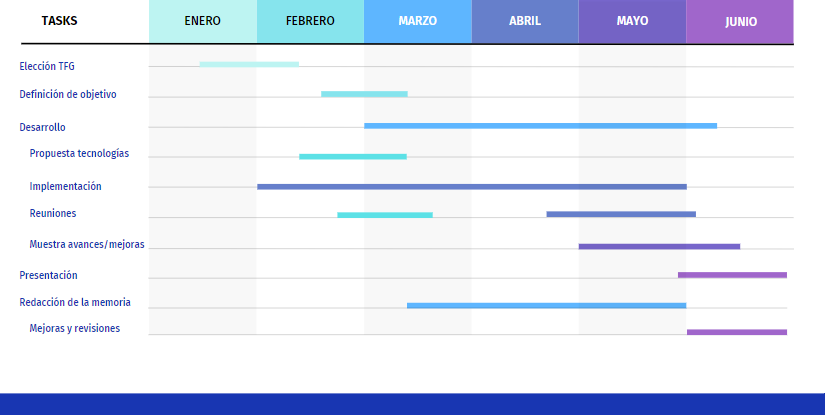
\includegraphics[width=\textwidth]{img/GANTT_TFG.png}
        \caption{Diagrama planificación temporal del proyecto}
        \label{figura:GANTT_TFG}
    \end{figure}
    
%%Lo importante es que quede claro cuánto tiempo has consumido en realizar el TFG/TFM 
%(tiempo natural, p.ej., 6 meses) y a qué nivel de esfuerzo (p.ej., principalmente los 
%fines de semana).


\section{Estructura de la memoria}
\label{sec:estructura}

Por último, en esta sección se introduce a alto nivel la organización del resto del documento
y qué contenidos se van a encontrar en cada capítulo.

    \begin{itemize}
      \item En este primer capítulo se hace una breve introducción al proyecto, presentando el contexto, se hace una descripción de los objetivos del mismo y se refleja la planificación temporal.
      \item En el siguiente capítulo se describen las tecnologías involucradas en el desarrollo de este proyecto. (Capítulo~\ref{chap:tecnologias}).
      \item En el capítulo~\ref{chap:diseño} se presentan los \textit{dataset} utilizados en el proyecto, explicando el esquema de la base de datos. 
      \item En el capítulo~\ref{chap:experimentos} se presentan las principales pruebas realizadas y se comentan los resultados de los experimentos
      efectuados por cada herramienta. 
      \item Por último, las principales conclusiones se presentan en el capítulo (Capítulo~\ref{chap:conclusiones}), incluyendo un resumen de las conclusiones obtenidas del proyecto, así como los trabajos futuros que podrían derivarse de éste.
    \end{itemize}


\section{Github}
\label{sec:github}
%A continuación, se puede visualizar el cronograma de este Trabajo Fin de Grado.

El código realizado para este Trabajo de Fin de Grado ha sido almacenado en un repositorio de Github\footnote{\url{https://github.com/crisgh/TFG-CristinaGallegoHerrero}}. Github \footnote{\url{https://docs.github.com/}} es es un servicio web que almacena repositorios de proyectos que utilizan el sistema de control de versiones Git.


\clearpage

%%%%%%%%%%%%%%%%%%%%%%%%%%%%%%%%%%%%%%%%%%%%%%%%%%%%%%%%%%%%%%%%%%%%%%%%%%%%%%%%
%%%%%%%%%%%%%%%%%%%%%%%%%%%%%%%%%%%%%%%%%%%%%%%%%%%%%%%%%%%%%%%%%%%%%%%%%%%%%%%%
% ESTADO DEL ARTE %
%%%%%%%%%%%%%%%%%%%%%%%%%%%%%%%%%%%%%%%%%%%%%%%%%%%%%%%%%%%%%%%%%%%%%%%%%%%%%%%%

\chapter{Estado del arte}               %% a.k.a "Tecnologías utilizadas"
\label{chap:tecnologias}

Para el desarrollo de este proyecto se han utilizado diferentes tecnologías, las cuales se explican en este capítulo.

\section{Atom} 
\label{sec:atom}
Atom\footnote{\url{https://atom.io/}} es un editor de código fuente especializado en la programación. Compatible con los lenguajes más populares, permite escribir código y programar desde tu PC con Windows, Linux o macOS, con soporte para múltiples \gls{plugin} escritos en Node.js y control de versiones Git integrado, desarrollado por GitHub. 

La mayor parte de los paquetes tienen licencias de software libre y está desarrollados y mantenidos por la comunidad de usuarios. Atom está basado en Electron (Anteriormente conocido como Atom Shell), un framework que permite crear aplicaciones de escritorio multiplataforma. También puede ser utilizado como un \gls{ide}.

\begin{figure}[ht]
        \centering
        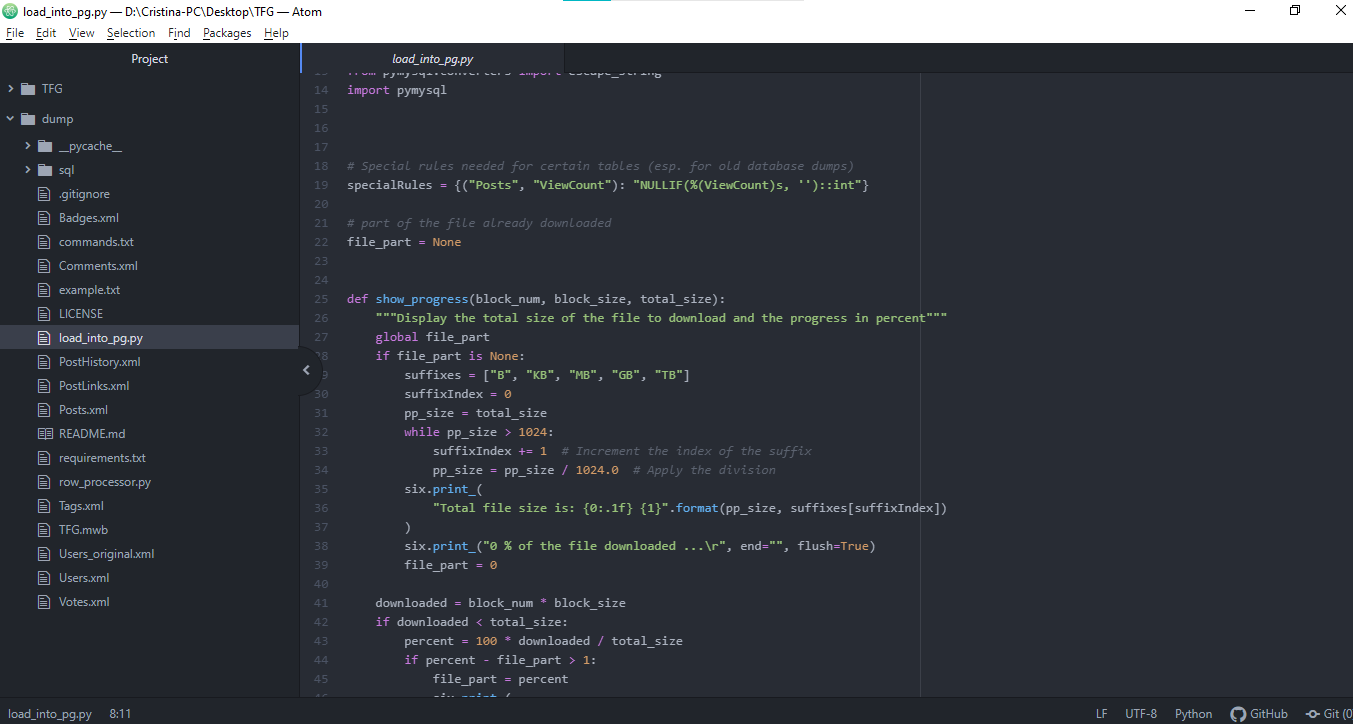
\includegraphics[width=\textwidth]{img/ATOM.png}
        \caption{Interfaz de Atom}
        \label{figura:ATOM}
    \end{figure}

Personalmente, he optado por Atom porque es el editor que suelo utilizar para todos
mis proyectos tanto personales como laborales. 

\section{Python} 
\label{sec:Python}

Python~\cite{van2007python} es un lenguaje de programación interpretado y dinámico, de código abierto \gls{oss}, que
soporta tanto el paradigma de la programación orientada a objetos (OOP) como el de la programación funcional.

Se ha elegido este lenguaje de programación para el parseado de datos extraídos de la plataforma de Stack Exchange\footnote{\url{https://stackexchange.com/}}. Además, Python, ofrece múltiples paquetes para la conexión con bases de datos. En este proyecto se ha utilizado el conector oficial de Oracle para MySQL, mysql-connector-python\footnote{\url{https://dev.mysql.com/doc/connector-python/en/connector-python-introduction.html}}, que cumple con la DB API 2.0 de Python~\cite{Python}.

\section{MySQL} 
\label{sec:Mysql}

El sistema gestor de la base de datos elegido para dar soporte a la persistencia de la información y el tratamiento de datos de forma conveniente ha sido MySQL (v8.0)~\cite{MYSQL}.

MySQL es uno de los gestores de bases de datos \gls{sql} más popular en la actualidad. Es desarrollado, distribuido y soportado por Oracle. Se trata de un \gls{oss}, que permite que pueda ser modificado dependiendo de las necesidades de cada usuario. El software de MySQL está basado en GPL (GNU General Public License) que define qué y qué no se debe hacer con el software en diferentes situaciones.

MySQL, desde la versión 5.6, proporciona una herramienta denominada  \textit{MySQLWorkbench}~\cite{krogh2020mysql}. Es una herramienta visual de diseño de bases de datos que integra desarrollo de software, administración de bases de datos, diseño de bases de datos, gestión y mantenimiento para el sistema de base de datos MySQL.

Se ha utilizado MySQL ya que es un source nativo tanto en Grafana como en Tableau, además ofrece múltiples ventajas, donde podemos destacar su alto rendimiento, bajo consumo de recursos, soporte a múltiples Sistemas Operativos y una alta securización de los datos.

\section{Tecnologías de visualización y análisis} 
\label{sec:Tenologias_va}
\subsection{Grafana/ Graphite} 
\label{sec:Grafana} 

\textbf{Grafana}~\cite{chakraborty2021grafana} es una herramienta \gls{oss} para la obtención de datos, almacenamiento, visualización y análisis.
Se conecta con todas las fuentes de datos posibles, como \textit{Graphite, Prometheus, Influx DB, ElasticSearch, MySQL, PostgreSQL}, y otros.

Grafana, mediante peticiones SQL en tiempo real a la Base de Datos, representa la
información obtenida en Paneles, que se considera cualquier elemento que represente de forma gráfica la información, y Dashboards, que se trata de una agrupación de paneles, de distinto tipo como, por ejemplo, gráficas de tiempo, sectores circulares, diagramas de barras, tablas, mapas, etc.

En la imagen \ref{figura:Grafana} se muestra  el panel principal de la interfaz gráfica de Grafana tras haber realizado el \emph{login} con usuario y contraseña.

\begin{figure}[ht]
        \centering
        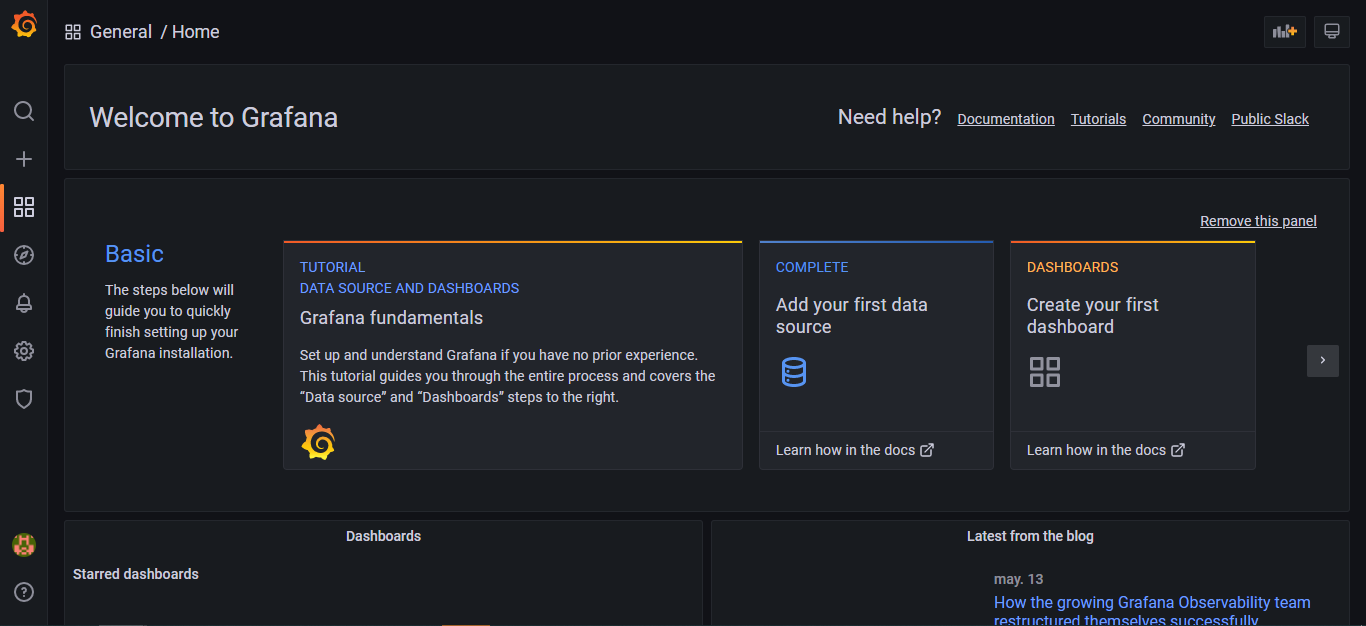
\includegraphics[width=0.8\textwidth]{img/Grafana.png}
        \caption{Interfaz gráfica Grafana}
        \label{figura:Grafana}
    \end{figure}

Uno de los complementos más utilizados de manera conjunta en Grafana es Graphite.
\textbf{Graphite} ~\cite{Graphite} es una herramienta de monitoreo. Facilita el almacenamiento y visualización de datos de series temporales. Idealmente, Graphite se usa como fuente de datos para el tablero de Grafana en una configuración de monitoreo de datos.

Graphite fue diseñado y escrito originalmente por Chris Davis en Orbitz en 2006 como un proyecto paralelo que finalmente se convirtió en su herramienta de monitoreo fundamental. En 2008, Orbitz permitió que Graphite se lanzara bajo la licencia de código abierto Apache 2.0 . Numerosas empresas grandes han implementado Graphite en la producción, donde les ayuda a monitorear sus servicios de comercio electrónico de producción y planificar el crecimiento.

\subsection{Tableau}
\label{sec:tableau}

Tableau~\cite{Tableau} es un software para el análisis y visualización de datos. Tableau se fundó en 2003 como resultado de un proyecto de ciencias de la computación de Stanford. Este tenía como objetivo mejorar el flujo del análisis y poner los datos al alcance de las personas a través de la visualización.  
Tableau destaca por su facilidad para integrar diferentes tipos de datos y permite la creación de dashboards que simplifican la toma de decisiones a partir de la información generada. Se trata de un programa flexible, ya que puede ser configurado para que trabaje bajo un servidor, en el escritorio o en la nube, visualizando los datos desde el principio. Además, ofrece cientos de conectores nativos para extraer, limpiar y correlacionar fácilmente datos de prácticamente cualquier fuente sin tener que crear un código personalizado.

En este proyecto, se han utilizado dos herramientas que ofrece Tableau: Tableau Prep (\ref{figura:Tableau_Prep}) y Tableau Desktop (\ref{figura:Tableau_desktop}). El primero, permite transformar y limpiar los datos mediante un proceso totalmente automático. El segundo, la aplicación principal, lleva a cabo todo el análisis y la creación de visualizaciones. 

\begin{figure}[ht]
    \centering
        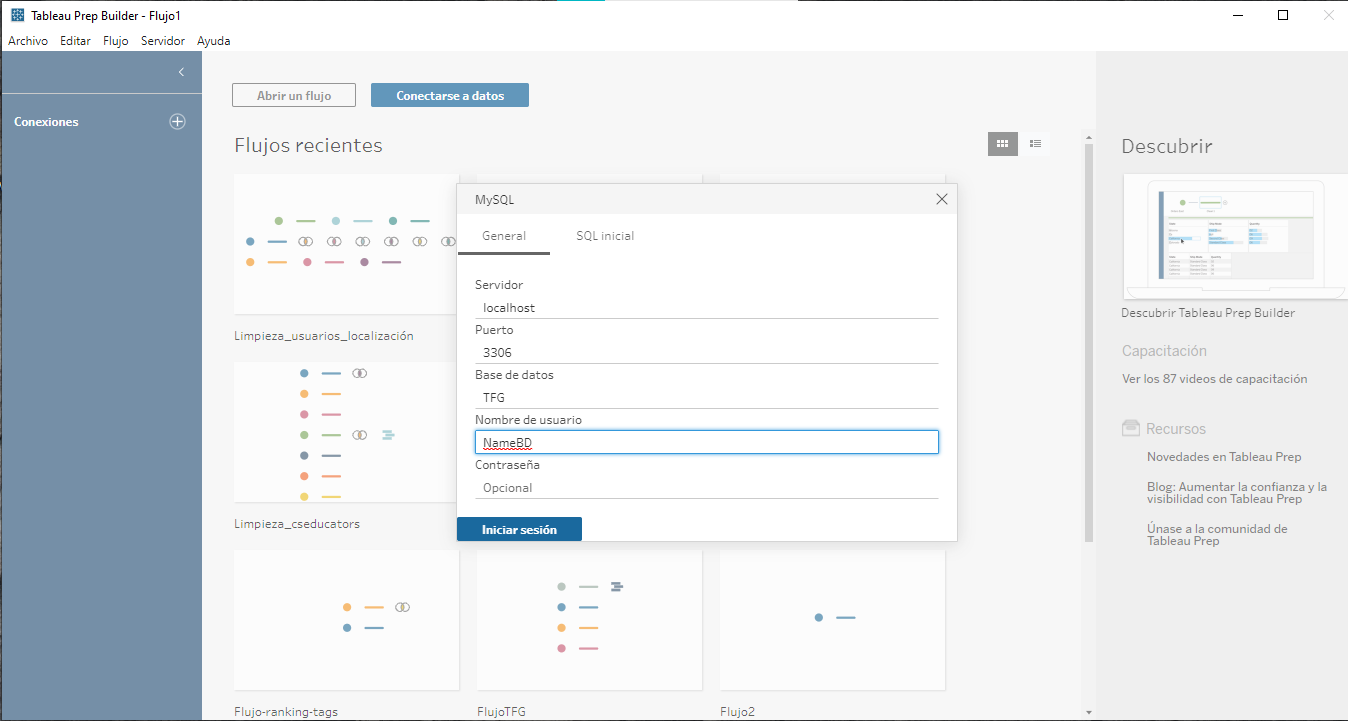
\includegraphics[width=0.8\textwidth]{img/PREP.png}
        \caption{Interfaz gráfica Tableau Prep}
        \label{figura:Tableau_Prep}
    \end{figure}

\begin{figure}[ht]
 \centering
  \subfloat[Connect Desktop]{
   \label{f:tableau}
    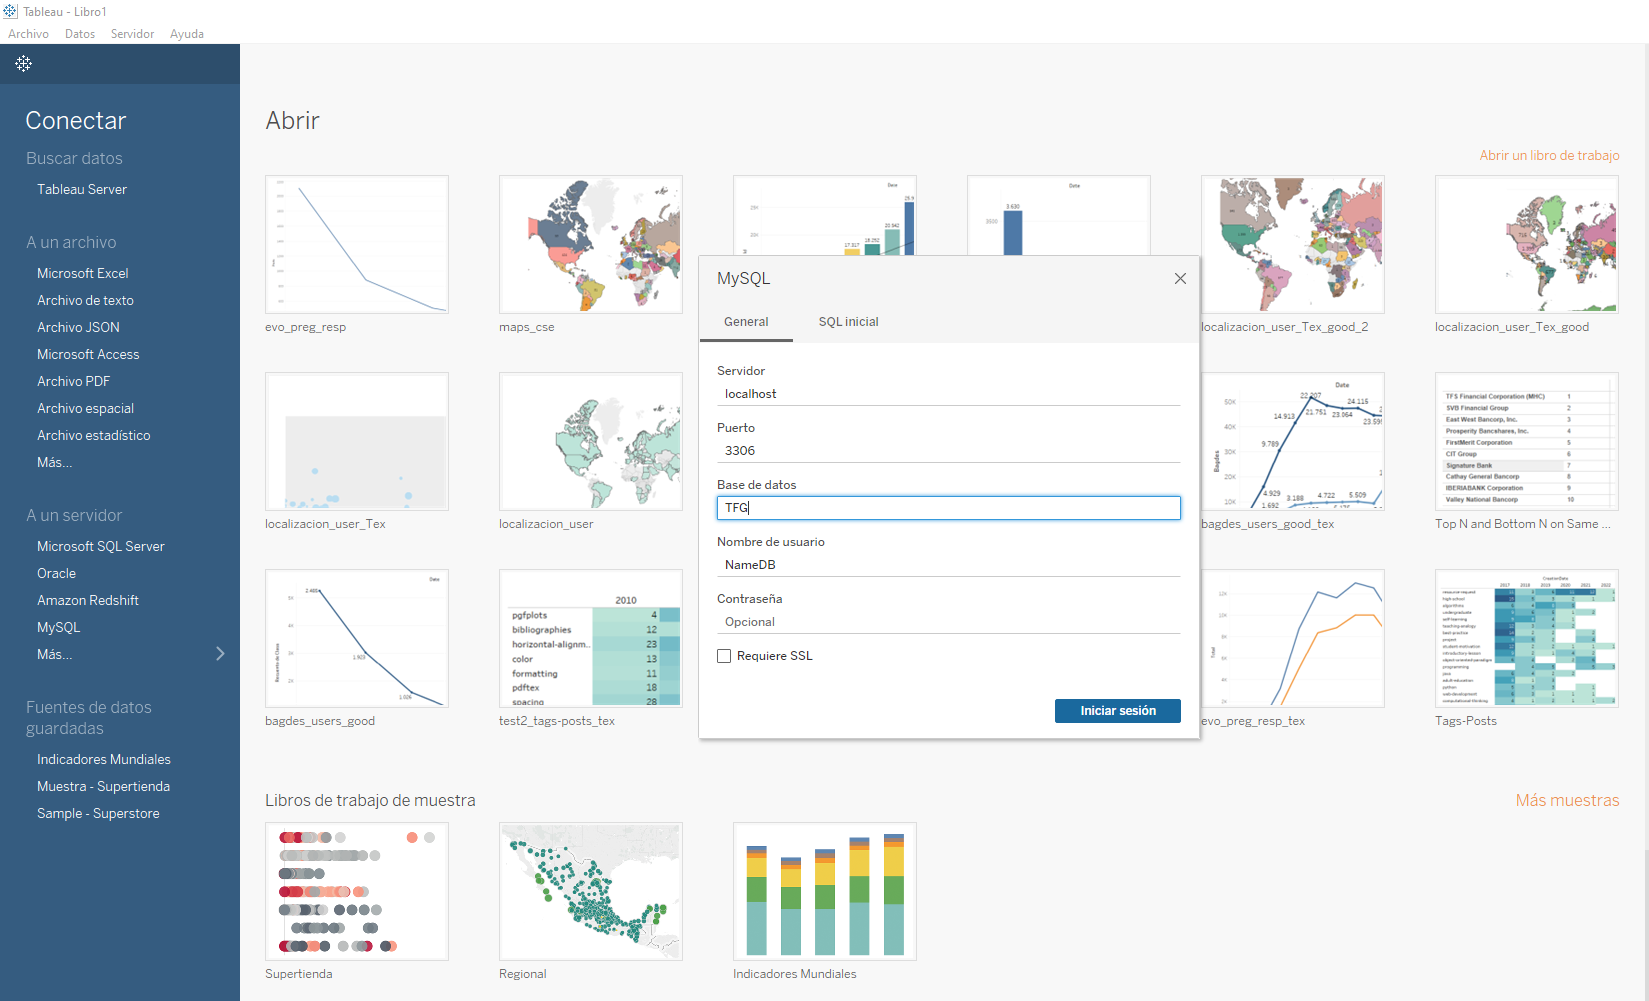
\includegraphics[width=0.4\textwidth]{img/Tableau_desktop.png}}
  \subfloat[Desktop]{
   \label{f:desktop}
    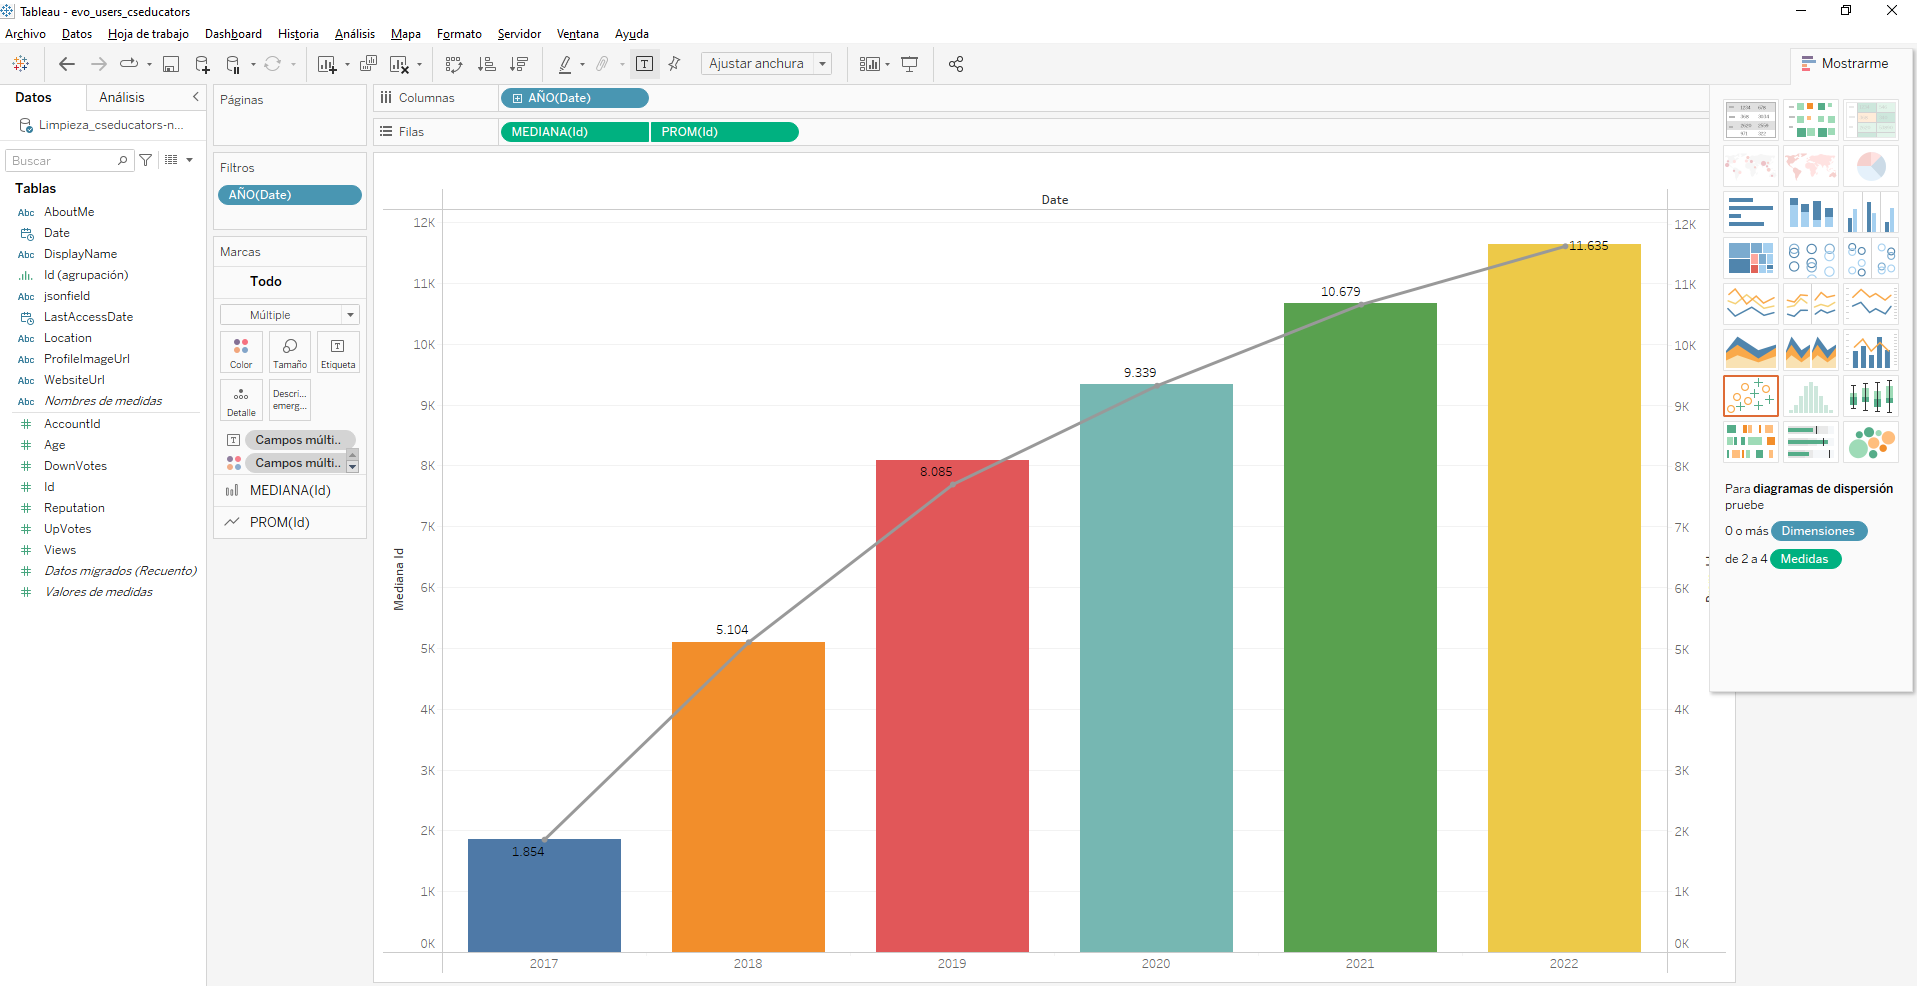
\includegraphics[width=0.4\textwidth]{img/Desktop.png}}
 \caption{Interfaz gráfica Tableau Desktop}
 \label{figura:Tableau_desktop}
\end{figure}
    
\section{Comparativa Side by Side}
\label{sec:comparativa}

Grafana y Tableau son herramientas para el análisis y visualización de datos. 

Por un lado, Grafana es un software de código abierto que fue diseñada para la visualización de series temporales, puede definirse como una "plataforma de observación". 
Esta herramienta presenta un panel principal (dashboard) que contiene diferentes visualizaciones de datos. Ofrece soporte nativo para una gran variedad de fuentes de datos, como InfluxDB, MySQL, PostgreSQL\ldots, además de integraciones con Prometheus y Graphite, herramientas de monitorización de series temporales. 

Por otro lado, Tableau es un software propietario diseñado principalmente en el marco empresarial. Permite extraer los datos de cualquier fuente, combinarlos y realizar transformaciones para preparar los datos para la visualización. 

Ambas presentan semejanzas, como puede ser el uso de tableros y técnicas de visualización más usuales, como gráficos de barras, histogramas, gráficos circulares o de dispersión. Permiten también valores únicos, tablas de texto, etc.   

Cada herramienta presenta sus propias características. %Además de las similitudes indicadas, 
Nos centraremos en las diferencias que ofrecen para definir una serie parámetros de comparación. 
\begin{itemize}
    \item \textbf{Usabilidad vía {\gls{gui}}}: Esta característica determina la facilidad de uso de cada herramienta. Describe que interfaz de usuario es más fácil de usar. 
    \item \textbf{Uso principal}: Especificaciones de uso habituales. 
    \item \textbf{Conjunto de datos}: Tamaño de las muestras procesadas.
    \item \textbf{Visualización}: Las opciones de visualización de datos es una de las características más importantes entre las diferentes herramientas. 
    \item \textbf{Licenciamiento y costes}: Términos y condiciones para el uso de la herramienta, además diferenciar el coste ya que el software puede ser gratuito o de pago. 
\end{itemize}


\section{Redacción de la memoria: LaTeX/Overleaf}
\label{sec:redaccion_de_la_memoria}

LaTeX es un sistema de composición tipográfica de alta calidad que incluye características especialmente diseñadas para la producción de documentación técnica y científica. Estas características, entre las que se encuentran la posibilidad de incluir expresiones matemáticas, fragmentos de código, tablas y referencias, junto con el hecho de que se distribuya como software libre, han hecho que LaTeX se convierta en el estándar de facto para la redacción y publicación de artículos académicos, tesis y todo tipo de documentos científico-técnicos. 

Por su parte, Overleaf es un editor LaTeX colaborativo basado en la nube. Lanzado originalmente en 2012, fue creado por dos matemáticos que se inspiraron en su propia experiencia en el ámbito académico para crear una solución satisfactoria para la escritura científica colaborativa.

Además de por su perfil colaborativo, Overleaf destaca porque, pese a que en LaTeX el escritor utiliza texto plano en lugar de texto formateado (como ocurre en otros procesadores de texto como Microsoft Word, LibreOffice Writer y Apple Pages), éste puede visualizar en todo momento y paralelamente el texto formateado que resulta de la escritura del código fuente.

\clearpage

%%%%%%%%%%%%%%%%%%%%%%%%%%%%%%%%%%%%%%%%%%%%%%%%%%%%%%%%%%%%%%%%%%%%%%%%%%%%%%%%
%%%%%%%%%%%%%%%%%%%%%%%%%%%%%%%%%%%%%%%%%%%%%%%%%%%%%%%%%%%%%%%%%%%%%%%%%%%%%%%%
% DISEÑO E IMPLEMENTACIÓN %
%%%%%%%%%%%%%%%%%%%%%%%%%%%%%%%%%%%%%%%%%%%%%%%%%%%%%%%%%%%%%%%%%%%%%%%%%%%%%%%%

\chapter{Diseño e implementación}
\label{chap:diseño}

En esta sección se explicará el diseño e implementación del proyecto, comenzando por una visión general, y después desglosando cada una de las partes que se han implementado en el desarrollo del proyecto.

\section{Arquitectura general} 
\label{sec:arquitectura}

En la figura~\ref{fig:_arquitectura} se puede observar el diagrama de flujo del proyecto. Comenzamos con el volcado de datos desde la plataforma Stack Exchange \footnote{\url{https://archive.org/details/stackexchange}} y tras descargar los ficheros, realizamos el \emph{parseo} de los mismos para insertarlos en la~\gls{bbdd} MySQL del proyecto. El diagrama de entidad-relación (EER) de la base de datos se puede observa en la figura~\ref{fig:modelo_entidad_relacion}, donde vemos las diferentes tablas que almacenan la información.   
\begin{figure}
    \centering
    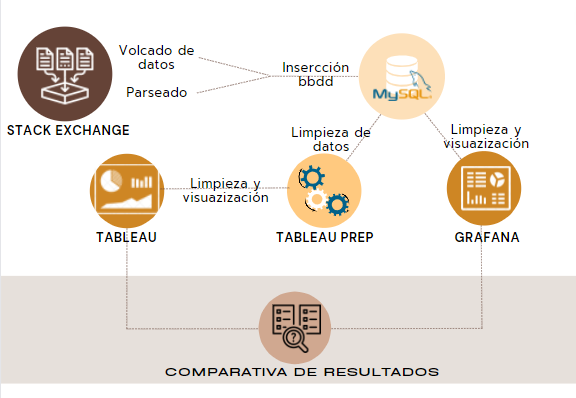
\includegraphics[width=0.7\textwidth, keepaspectratio]{img/flujo_arquitectura.png}
    \caption{Diagrama de flujo del proyecto}\label{fig:_arquitectura}
\end{figure}

\begin{figure}
  \centering
  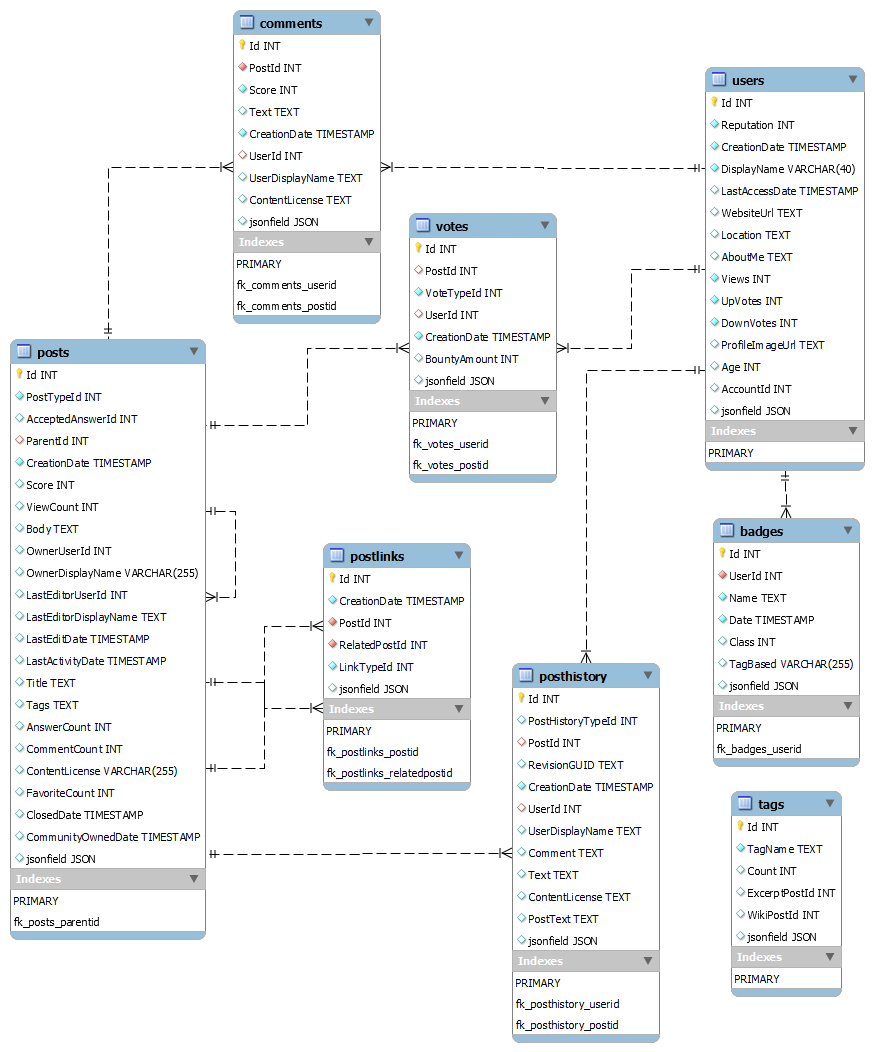
\includegraphics[width=0.5\textwidth, keepaspectratio]{img/modelo_entidad_relacion.png}
  \caption{Diagrama de entidad-relación (\gls{eer}) de la Base de Datos.}\label{fig:modelo_entidad_relacion}
\end{figure}

Veremos con más detalle el \emph{parseo} de datos en el capítulo \ref{sec:parser}, ya que se ha implementado un programa en Python que realiza la descarga y la inserción de datos en MySQL.

Una vez que tenemos los datos en nuestra~\gls{bbdd}, realizamos la conexión con las diferentes herramientas de análisis y visualización. En nuestro caso, conectamos la base de datos con Grafana y Tableau Prep. Desde Grafana, realizamos la limpieza de los datos, el análisis de estos y su visualización. La conexión con Tableau Prep nos permite llevar a cabo la limpieza de datos y conectamos directamente con Tableau Desktop que realiza su análisis y visualización.

Por último, en el flujo del proyecto, vemos la comparación de los resultados obtenidos en ambas herramientas basándonos en los criterios identificados en la sección \ref{sec:comparativa}

Cabe destacar que se ha utilizado MySQL como plataforma para alojar la base de datos por ser un \emph{source} nativo de las herramientas, es decir, podemos conectarnos a los datos sin desarrollos adicionales.

\subsection{Parseado de datos}
\label{sec:parser} 

Como se indicaba en el capitulo anterior, en este proyecto se ha implementado un \emph{parser} en Python encargado de transformar los datos \gls{xml} a la estructura de datos para ser procesada en MySQL. 

En la figura \ref{fig:proyecto-atom} observamos la estructura del proyecto. En ella encontramos el fichero \texttt{load\_into\_pg.py} que se trata del script principal. En este fichero se importan las diferentes librerías propias de python y el módulo \texttt{row\_processor.py} usado para analizar el fichero XML volcado de StackExchange y que devuelve un generador de campos por cada línea extraída. 

%
\begin{wrapfigure}{r}{0.25\textwidth} %this figure will be at the right
    \centering
    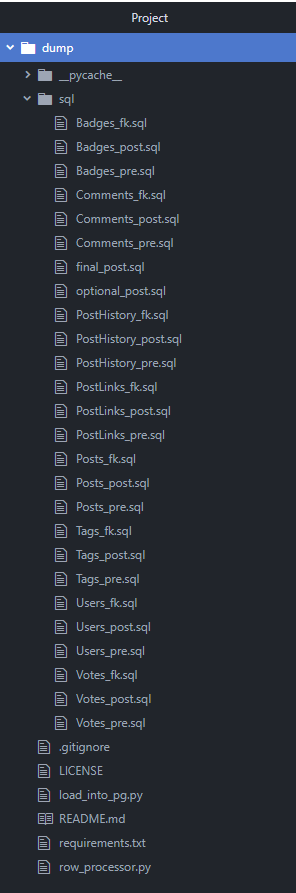
\includegraphics[width=0.24\textwidth]{img/proyecto-atom.png}
    \caption{Proyecto en Atom - Parseo de datos}\label{fig:proyecto-atom}
\end{wrapfigure}

Centrándonos en el fichero \texttt{load\_into\_pg.py}, presenta dos modalidades de uso: Una, realizando carga de la base de datos mediante la descarga de ficheros en un directorio temporal, que tras ser procesado será borrado. Otra, realizando la carga cada la tabla de la base de datos asociada por cada fichero extraído previamente en local. 

Si elegimos la descarga completa, haremos uso de la función \texttt{show\_progress} que muestra el tamaño total del archivo a descargar y el progreso en porcentaje. Es el único punto que difiere el código para la obtención de datos.

Siguiendo con el fichero, tenemos distintas llamadas a ficheros externos que generan las plantillas para la creación de las tablas.

La función principal \texttt{handleTable} maneja las diferentes tablas, incluyendo el preprocesado y el posprocesado, indicando el tiempo que se emplea en cada paso. Además,  realiza la conexión con la base de datos. En nuestro caso, como se ha indicado en capítulos previos, hemos utilizado MySQL y para conectarnos se ha hecho uso del conector \texttt{mysql.connector} (oficial de Oracle).

Para el preprocesado de datos, se hace referencia a los ficheros \texttt{\emph{nombre\_tabla}\_pre.sql} que incluye la \emph{query} para la creación de las distintas tablas. Una vez creadas, se realiza el procesado y la extracción de los diferentes elementos mediante el módulo \texttt{row\_processor.py} que parsea el XML. Tras ese parseado, desde el script principal, se lanza un bucle para recorrer todas las fichas que llama a la función \texttt{ins\_query\_maker} que asocia cada atributo (columnas) con las tuplas (Conjunto de filas) devueltas en el parseado y se crea la \emph{query} que sera retornada para que se ejecute desde la función principal.

\begin{listing}[t]
    \caption{Función: \texttt{ins\_query\_maker}.}{}
    \label{lst:1}
    \begin{minted}[breaklines, fontsize=\footnotesize, baselinestretch=1]{python}
def ins_query_maker(keys,cursor,tablename, rowdict,insertJson):
   
    keys = tuple(rowdict)
    dictsize = len(rowdict)
    sql = ''
    for i in range(dictsize) :
        if(type(rowdict[keys[i]]).__name__ == 'str'):
            sql += '\'' + str(rowdict[keys[i]].replace("'", "\\'")) + '\''
        else:
            sql += str(rowdict[keys[i]])
        if(i< dictsize-1):
            sql += ', '
    if insertJson:
        dict_attribs = {}
        for name, value in rowdict.items():
            dict_attribs[name] = value
        sql += ', \'' + str(escape_string(json.dumps(dict_attribs))) + '\''
        key = str(keys) + ', jsonfield'
        key = key.replace("'", "")
        key = key.replace(")", "")
        key = key + ")"
    else:
        key = str(keys)
        key = key.replace("'", "")

    query = "insert into " + str(tablename) + " " + key + " values (" + str(sql) + ");"
    return query
    \end{minted}
\end{listing}

Una vez procesados los datos, se realiza el posprocesado que referencia otros ficheros \texttt{\emph{nombre\_tabla}\_post.sql} y \texttt{\emph{nombre\_tabla}\_fk.sql} encargados de generar los índices y las referencias (\textit{foreign key}) de las tablas.  

\begin{listing}[t]
    \caption{Fichero para la creación de referencias: \texttt{Comments\_fk.sql}.}{}
    \label{lst:2}
    \begin{minted}[breaklines, fontsize=\footnotesize, baselinestretch=1]{sql}
SET FOREIGN_KEY_CHECKS = 0;
ALTER TABLE Comments ENGINE=InnoDB;
ALTER TABLE Users ENGINE=InnoDB;
ALTER TABLE Comments ADD CONSTRAINT fk_comments_userid FOREIGN KEY (userid) REFERENCES users (id);
ALTER TABLE Comments ADD CONSTRAINT fk_comments_postid FOREIGN KEY (postid) REFERENCES posts (id);
    \end{minted}
\end{listing}

Finalmente, tras lanzar el script obtenemos la base de datos completa y actualizada con los datos a analizar.

\begin{listing}[t]
    \caption{Tablas creadas en MySQL.}{}
    \label{lst:3}
    \centering
    \begin{minted}[breaklines, fontsize=\footnotesize, baselinestretch=1]{sql}
                                mysql> show full tables;
                                +---------------+------------+
                                | Tables_in_tfg | Table_type |
                                +---------------+------------+
                                | badges        | BASE TABLE |
                                | comments      | BASE TABLE |
                                | posthistory   | BASE TABLE |
                                | postlinks     | BASE TABLE |
                                | posts         | BASE TABLE |
                                | tags          | BASE TABLE |
                                | users         | BASE TABLE |
                                | votes         | BASE TABLE |
                                +---------------+------------+
    \end{minted}
\end{listing}

\begin{listing}[t]
    \caption{Tabla \texttt{Comments} en MySQL}{}
    \label{lst:4}
    \begin{minted}[breaklines, fontsize=\footnotesize, baselinestretch=1]{sql}
                mysql> desc comments;
                +-----------------+-----------+------+-----+---------+-------+
                | Field           | Type      | Null | Key | Default | Extra |
                +-----------------+-----------+------+-----+---------+-------+
                | Id              | int       | NO   | PRI | NULL    |       |
                | PostId          | int       | NO   | MUL | NULL    |       |
                | Score           | int       | NO   |     | NULL    |       |
                | Text            | text      | YES  |     | NULL    |       |
                | CreationDate    | timestamp | NO   |     | NULL    |       |
                | UserId          | int       | YES  | MUL | NULL    |       |
                | UserDisplayName | text      | YES  |     | NULL    |       |
                | ContentLicense  | text      | YES  |     | NULL    |       |
                | jsonfield       | json      | YES  |     | NULL    |       |
                +-----------------+-----------+------+-----+---------+-------+
    \end{minted}
\end{listing}
\begin{listing}[t]
    \caption{Foreign Key de la tabla \texttt{Comments} en MySQL}{}
    \label{lst:5}
    \begin{minted}[breaklines, fontsize=\footnotesize, baselinestretch=1]{sql}
    mysql> SELECT CONSTRAINT_CATALOG,CONSTRAINT_NAME,TABLE_NAME,CONSTRAINT_TYPE,ENFORCED FROM information_schema.TABLE_CONSTRAINTS
        -> WHERE information_schema.TABLE_CONSTRAINTS.CONSTRAINT_TYPE = 'FOREIGN KEY'
        -> AND information_schema.TABLE_CONSTRAINTS.TABLE_SCHEMA = 'tfg'
        -> AND information_schema.TABLE_CONSTRAINTS.TABLE_NAME = 'comments';
    +--------------------+--------------------+------------+-----------------+----------+
    | CONSTRAINT_CATALOG | CONSTRAINT_NAME    | TABLE_NAME | CONSTRAINT_TYPE | ENFORCED |
    +--------------------+--------------------+------------+-----------------+----------+
    | def                | fk_comments_postid | comments   | FOREIGN KEY     | YES      |
    | def                | fk_comments_userid | comments   | FOREIGN KEY     | YES      |
    +--------------------+--------------------+------------+-----------------+----------+
    \end{minted}
\end{listing}

\clearpage

\section{Datasets}
\label{sec:datasets}

Los datasets utilizados en este Trabajo de Fin de Grado han sido extraídos de la plataforma Stack Exchange \footnote{\url{https://stackexchange.com/}}, una plataforma compuesta por 173 comunidades online de preguntas y respuestas, que permite a los usuarios realizar preguntas, aprender y compartir conocimientos.

El contenido de los dataset esta organizado en varias tablas: 
 \begin{itemize}
        \item \emph{Badges} - Insignias, es la reputación del usuario en la comunidad de Stack Exchange (oro, plata,bronce\ldots)
        \item \textbf{\emph{Comments}} - Comentarios de la publicación.
        \item \textbf{\emph{Posthistorys}} - Historial de la publicación.
        \item \textbf{\emph{Postlinks}} - Enlaces a la publicación (vinculado/duplicado).
        \item \textbf{\emph{Posts}} - Publicaciones realizadas.
        \item \textbf{\emph{Tags}} - Etiquetas, relacionadas con la publicación.
        \item \textbf{\emph{Users}} - Usuarios únicos de la comunidad. 
        \item \textbf{\emph{Votes}} - Votos (Favorito, ofensivo, \emph{spam}, etc.) asociados a la publicación. 
    \end{itemize}

\subsection{Primer dataset: Computer Science Educators}
\label{sec:cseducators} 
Como dataset inicial, para realizar una comparativa de los datos obtenidos en ambas herramientas, se ha elegido uno de pequeñas dimensiones. En este caso ha sido Computer Science Educators (\emph{cseducators}).

Computer Science Educators\footnote{\url{https://cseducators.stackexchange.com/}}, es un servicio web de pregunta-respuesta de Stack Exchange para Educadores de Ciencias de la Computación, es decir, para aquellas personas involucradas en el campo de la enseñanza de las Ciencias de la Computación. Hay unos diez mil usuarios utilizando la plataforma y es visitada por unos 84 usuarios al día.

Este dataset ha sido elegido por el número de usuarios de la plataforma y la cantidad de preguntas existentes, que es aproximadamente de mil preguntas/respuestas. 

%%\subsection{Segundo dataset: Chemistry}
%\label{sec:chemistry} 
%*******  superuser.com.7z
%*******  math.stackexchange.com.7z
%*******  apple.stackexchange.com.7z
%*******  tex.stackexchange.com.7z

\subsection{Segundo dataset: Tex}
\label{sec:tex} 
Como segundo dataset se ha elegido uno de mayores dimensiones, que incluye una extensa cantidad de datos extraídos de la plataforma Tex StackExhange (\emph{tex}).

Tex \footnote{\url{https://https://tex.stackexchange.com/}} es parte de la red Stack Exchange. se trata de un sitio web de preguntas y respuestas para usuarios de Tex, LaTeX, ConTeXt y otros sistemas de tipografía y composición de documentos. La plataforma fue fundada en 2010 y es una comunidad activa, con unas 235 mil preguntas y más de 300 mil respuestas. El número de usuarios es más de 230 mil y es visitada por, aproximadamente, 58 mil de usuarios al día.

Se ha escogido este dataset por el número de usuarios de la plataforma y la cantidad de preguntas existentes, ya que representa una comunidad de gran tamaño. 

\cleardoublepage

%%%%%%%%%%%%%%%%%%%%%%%%%%%%%%%%%%%%%%%%%%%%%%%%%%%%%%%%%%%%%%%%%%%%%%%%%%%%%%%%
%%%%%%%%%%%%%%%%%%%%%%%%%%%%%%%%%%%%%%%%%%%%%%%%%%%%%%%%%%%%%%%%%%%%%%%%%%%%%%%%
% EXPERIMENTOS Y VALIDACIÓN %
%%%%%%%%%%%%%%%%%%%%%%%%%%%%%%%%%%%%%%%%%%%%%%%%%%%%%%%%%%%%%%%%%%%%%%%%%%%%%%%%

\chapter{Experimentos y validación}
\label{chap:experimentos}

En este capítulo se describen paso a paso los experimentos implementados por cada Dataset de nuestro proyecto, las representaciones con las que analizaremos el comportamiento de las herramientas en función de los criterios identificados en los apartados previos y la evolución de las comunidades. 

\section{Experimento Computer Science Educators}
\label{chap:exper_cseducators}

Para comenzar con el experimento, seguimos el flujo mencionado en el apartado \ref{sec:arquitectura}. 
Primero crearemos la base de datos (\emph{cseducators}) en MySQL que utilizaremos en este experimento \ref{lst:7}. Después lanzaremos el script \texttt{load\_into\_pg.py} que descarga los ficheros, parsea los datos y los carga sobre la base creada.
\begin{listing}[t]
    \caption{Create database}{}
    \label{lst:7}
    \begin{minted}[breaklines, fontsize=\footnotesize, baselinestretch=1]{sql}
                        mysql> create database cseducators;
                        Query OK, 1 row affected (0.04 sec)
    \end{minted}
\end{listing}

Con el dataset extraído de Stack Exchange indicado anteriormente, se ha decidido realizar una serie de visualizaciones, descritas en las siguientes secciones, que nos permiten analizar la comunidad y visualizarlas mediante el uso de ambas herramientas. 


\subsection{Usuarios}
Dentro de este dataset, una de las métricas más importantes es el número de usuarios que utilizan la plataforma. Cada usuario presenta un identificador único dentro de la comunidad.  
Esta comunidad fue creada en 2017, por lo que los primeros usuarios son de esa fecha. A partir de ese momento el número de usuarios se ve incrementado hasta la fecha actual. 

Se puede representar el valor de los usuarios de diversas formas: mostrando el total de usuario existentes, o mostrando la evolución y el crecimiento que han tenido durante diferentes periodos temporales. 

Los datos descargados tienen una fecha de extracción del 17 de marzo de 2022, hasta este día hay un total de 10475 usuarios. Podemos observar ese dato gráficamente en la figura  \ref{figura:total_users}. 

\begin{figure}[ht]
    \centering
    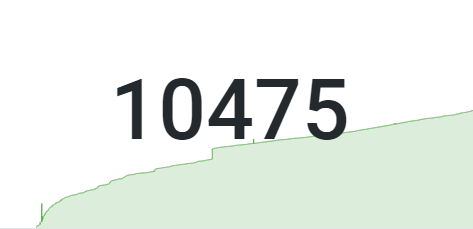
\includegraphics[width=0.5\textwidth]{img/cse/Total_usuarios.png}
    \caption{Panel: Total de usuarios (Interfaz: Grafana)}
    \label{figura:total_users}
\end{figure}


Este dato nos aporta una visión general pero no permite observar la evolución de la plataforma. Para ello, se procede a generar otra visualización que desglosa estos datos por años, visualizando así la evolución total de la comunidad.

\begin{figure}[ht]
    \centering
    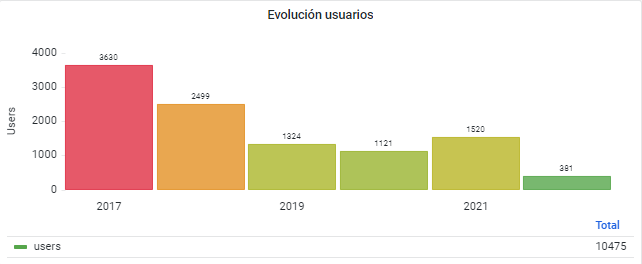
\includegraphics[width=0.75\textwidth]{img/cse/evolucion_usuarios.png}
    \caption{Panel: Evolución anual de usuarios (Interfaz: Grafana)}
    \label{figura:evo_users}
\end{figure}

Como se puede observar en la figura \ref{figura:evo_users} el registro de usuarios es mucho más elevado cuando se creó la comunidad y tras ese primer periodo, se puede observar que el número de usuarios que ingresan en la comunidad es mucho menor, estabilizándose en los últimos años.

Continuamos desglosando la información, para mostrar los datos agrupados en meses y podemos observar que existen periodos de mayor actividad.

Si vemos detenidamente la gráfica \ref{figura:evo_users_trim} observamos que una vez que se estabiliza la comunidad, a partir de 2019, se observa que existe un mayor registro de usuarios en los periodos lectivos, siendo el tercer trimestre el que menor número de usuarios registra. 

\begin{figure}[ht]
    \centering
    \includegraphics[width=0.6\textwidth]{img/cse/evolucion_usuarios_años.png}
    \caption{Panel: Evolución trimestral de usuarios (Interfaz: Tableau)}
    \label{figura:evo_users_trim}
\end{figure}

Con los datos extraídos y analizados en la herramienta de Tableau, podemos realizar un pronóstico de crecimiento de la plataforma siguiendo la tendencia existente. Esta información se muestra en la gráfica \ref{figura:tendencia_cse}, según este modelo el número de nuevos usuarios seguirá descendiendo.

\begin{figure}[ht]
    \centering
    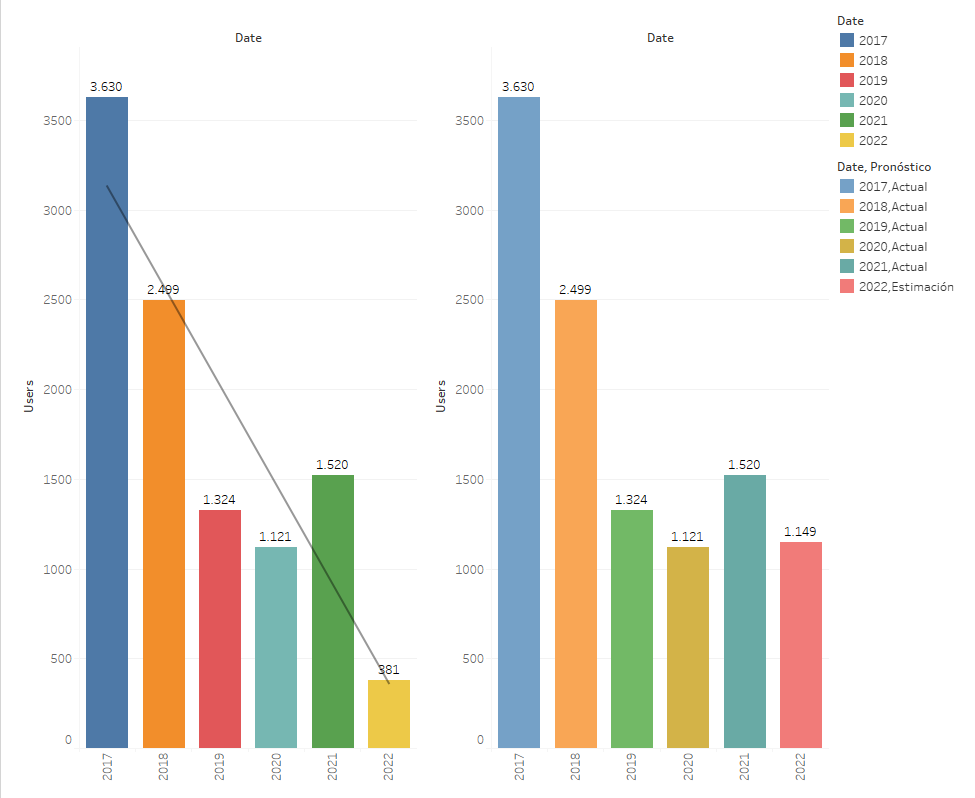
\includegraphics[width=0.6\textwidth]{img/cse/Tendencia_pronostico_CsE.png}
    \caption{Panel: Tendencia y pronóstico 2022 CS Educators (Interfaz: Tableau)}
    \label{figura:tendencia_cse}
\end{figure}




Entre el conjunto de datos existente en la tabla de usuarios se encuentra la localización. Si observamos la figura \ref{figura:MAP_users_cse} vemos los países presentan mayor cantidad de usuarios. En este dataset tenemos aproximadamente dos mil usuarios con localización distinta de \emph{NULL} por ello se ha realizado un preprocesado de estos datos para unificar los datos y excluir todos los valores que no contienen una ubicación real. 

\begin{figure}[ht]
    \centering
    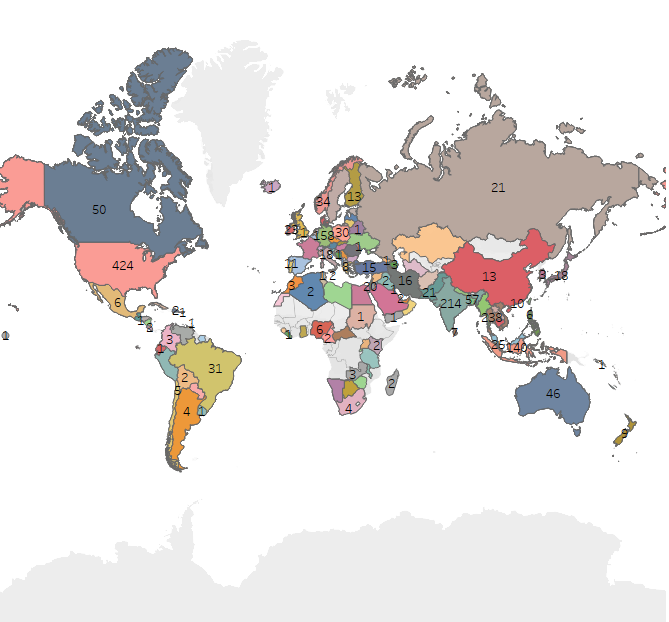
\includegraphics[width=0.75\textwidth]{img/cse/Maps_cse.png}
    \caption{Panel: Localización de usuarios Tex (Interfaz: Tableau)}
    \label{figura:MAP_users_cse}
\end{figure}


\subsection{Publicaciones}
Otra métrica habitual dentro de las comunidades de pregunta/respuesta, son las publicaciones realizadas, ya que nos permiten identificar como va consolidándose en el tiempo. 

En la gráfica \ref{figura:evo_post_anual} observamos que el número de preguntas al comienzo es muy elevado, en ese momento las preguntas que puedan surgir empiezan a aparecer en la comunidad por los diferentes usuarios. Tras el primer año de la plataforma el número disminuye significativamente, ya que muchas de las posibles preguntas pueden encontrarse ya publicadas. 

\begin{figure}[ht]
    \centering
    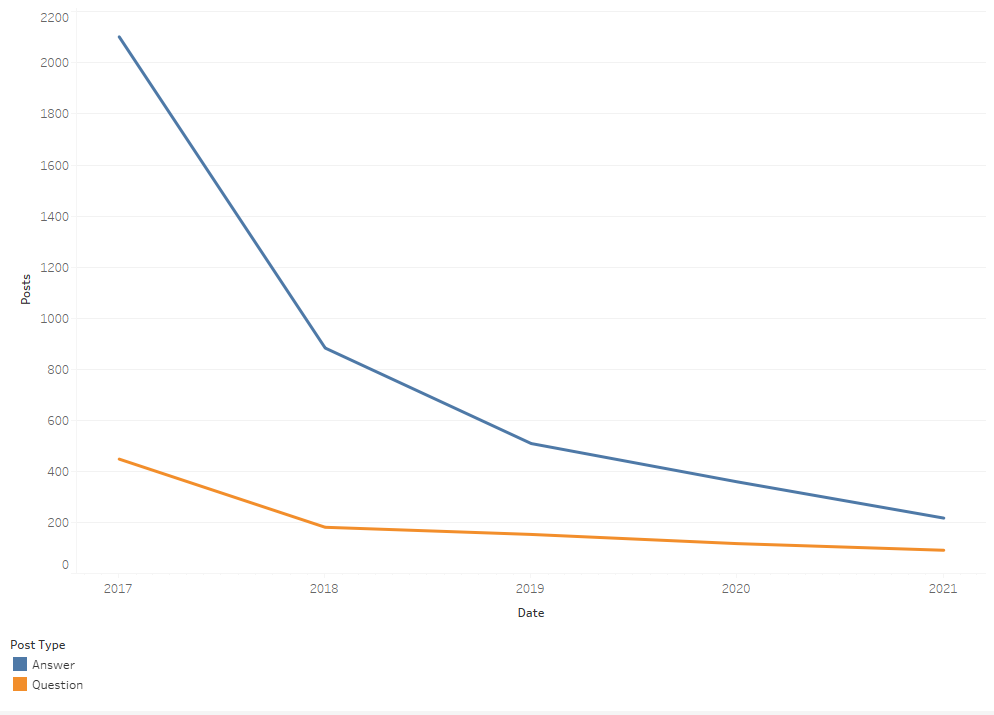
\includegraphics[width=0.8\textwidth]{img/cse/evo_posts_anual.png}
    \caption{Panel: Evolución pregunta/respuesta (Interfaz: Tableau)}
    \label{figura:evo_post_anual}
\end{figure}

Podemos ver en la figura \ref{fig:Pq_an} estos valores visualizando en forma de tabla el total de preguntas y respuestas por cada año.

Dentro de la publicación se pueden obtener datos adicionales que se encuentran relacionados. Uno de estos valores sería la puntuación, que contabiliza el número de votos positivos menos el número de votos negativos, obteniendo así el valor que presenta la publicación. 

\begin{figure}
    \begin{minipage}[b]{0.45\linewidth}
        \centering
        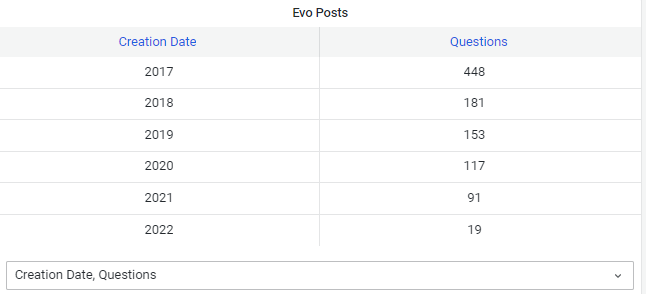
\includegraphics[width=\textwidth]{img/cse/evo_posts_questions.png}
        \end{minipage}
    \hspace{0.5cm}
    \begin{minipage}[b]{0.45\linewidth}
        \centering
        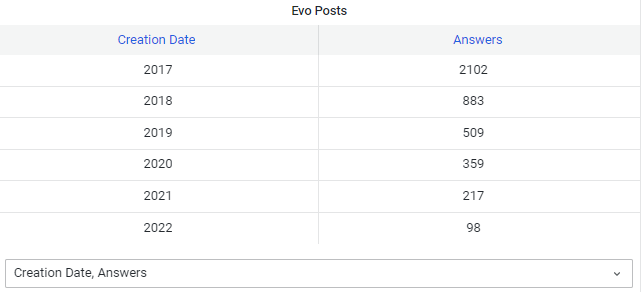
\includegraphics[width=\textwidth]{img/cse/evo_posts_answers.png}
    \end{minipage}
    \caption{Evolución preguntas/respuestas anuales (Interfaz Grafana)}
    \label{fig:Pq_an}
\end{figure}



Dentro de las publicaciones también podemos ver el indicador de favoritos, que contabiliza el número de veces que una publicación ha sido guardada por los usuarios de la plataforma. En la tabla \ref{table:top_5_cseducators} podemos ver un ejemplo del top 5 de los \emph{posts} con mayor número de favoritos de la comunidad con el \emph{link} al post y la puntuación otorgada por los usuarios y su título. 
\begin{table}[ht]
\centering
    \begin{tabular}{@{} p{2cm} p{6cm} p{1cm} p{2cm} @{}}
        \hline
        Post link & Title & Score & Favorite \\
        \hline
        5023 & Why do we count starting from zero? & 187 & 84 \\ 
        4425 & Should I teach that 1 kB = 1024 bytes or 1000 bytes?  & 138 & 40 \\ 
        3881 & Is there some meaningful percentage of students who can't learn to program? & 113 & 37 \\ 
        4197 & How to explain the concept of a variable to a 9-year old? & 90 & 33 \\ 
        4717 & Is it better to lie to students or to be pedantic when teaching Intro CS? & 123 & 28 \\ 
        \hline
    \end{tabular}
\caption{Top 5 Publicaciones favoritas de la comunidad CS Educators}
\label{table:top_5_cseducators}
\end{table}


%
%

\subsection{Tags}

Las etiquetas de una publicación son las diferentes palabras o conjunto de palabras que identifican el tema relacionado con la publicación. Es un medio de conexión entre las preguntas y los expertos. También suelen usarse para identificar preguntas interesantes o relevantes para los usuarios de la comunidad. 

Una de las bases es que como límite cada pregunta solo puede contener un máximo de 5 etiquetas. De manera general, se debe evitar la creación de nuevas etiquetas dentro de la comunidad. Existe un formateo en las etiquetas como el uso de minúsculas, reemplazo de espacios por guiones, evitar signos de puntuación o uso de nombres habituales, que pueden ser abreviaturas.

En la figura \ref{figura:evo_tags_anual} vemos las etiquetas más populares de la comunidad de \emph{cseducadors} de forma individual, donde se ha extraído la información de cada etiqueta utilizada. 

Las etiquetas de la publicación sirven para realizar búsquedas más rápidas dentro de la comunidad. Por tanto, otra relación interesante es la existente entre las etiquetas y el número de visualizaciones de las publicaciones las contienen. En la figura \ref{figura:evo_tags} se representan las etiquetas más usadas sin esa separación de etiquetas y cuantas visualizaciones totales desde la creación de la comunidad hasta la actualidad han tenido. 

\begin{figure}[ht]
    \centering
    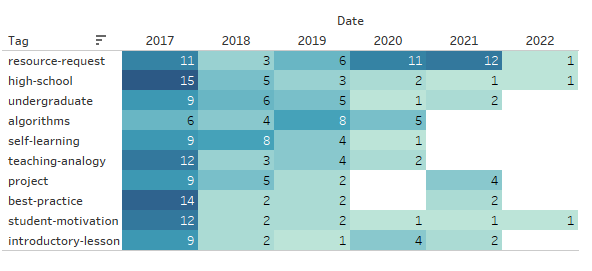
\includegraphics[width=0.5\textwidth]{img/cse/tags_evo.png}
    \caption{Panel: Evolución tags (Interfaz: Tableau)}
    \label{figura:evo_tags_anual}
\end{figure}

\begin{figure}[ht]
    \centering
    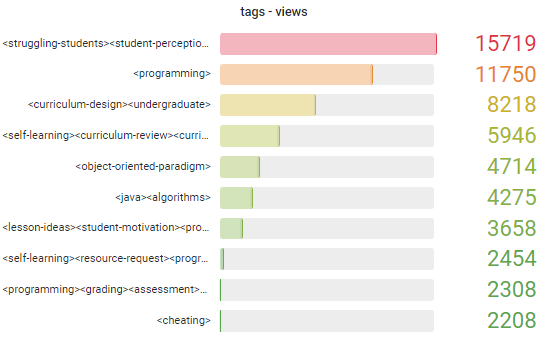
\includegraphics[width=0.5\textwidth]{img/cse/evo_tags.png}
    \caption{Panel: Evolución tags agregadas (Interfaz: Grafana)}
    \label{figura:evo_tags}
\end{figure}


Como es normal, las etiquetas y las visitas de una publicación dependen del periodo de tiempo que visualizamos. Por lo que la distribución varía de la fecha de publicación. En el gráfico \ref{figura:dist_tags} observamos las visualizaciones que presenta cada \emph{tag} individual por cada año. Si observamos las figuras \ref{figura:tags_2017} y \ref{figura:tags_2020} vemos que las etiquetas más usadas en cualquier periodo, ordenados por el conteo de visualizaciones que presentan estas etiquetas, no es semejante al resto de periodos. Las \emph{tags} más usadas en 2017 no se vuelen a usar prácticamente en el resto de años. Lo mismo ocurre por ejemplo si tratamos los datos de 2020, las publicaciones, preguntas o respuestas más visualizadas son totalmente diferentes y puede verse la tendencia de uso y el entorno en el que se realizan las publicaciones. 

\begin{figure}[ht]
    \centering
    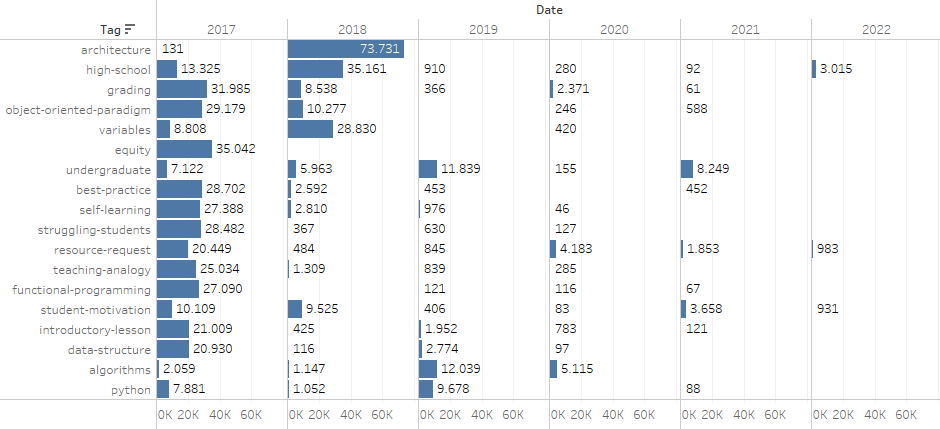
\includegraphics[width=\textwidth]{img/cse/tags_distrib.png}
    \caption{Panel: Distribución tags (Interfaz: Tableau)}
    \label{figura:dist_tags}
\end{figure}

\begin{figure}[ht]
    \centering
    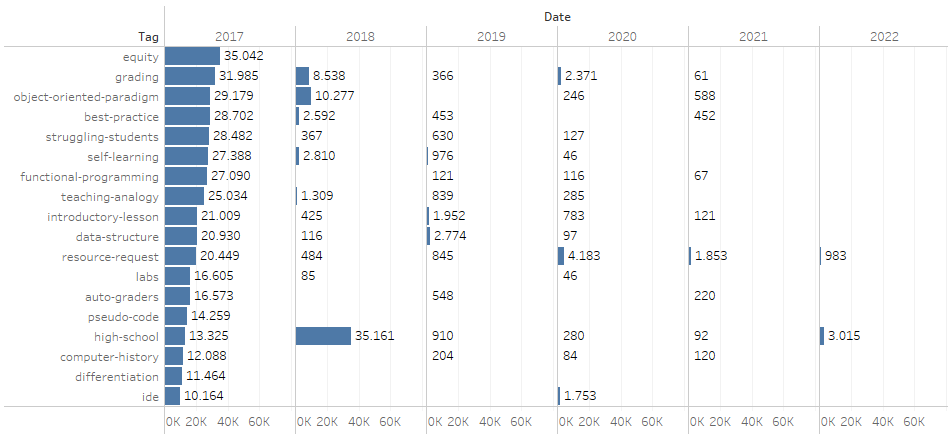
\includegraphics[width=\textwidth]{img/cse/tags_2017.png}
    \caption{ Distribución de etiquetas 2017 (Interfaz Tableau)}
    \label{figura:tags_2017}
\end{figure}

\begin{figure}[ht]
    \centering
    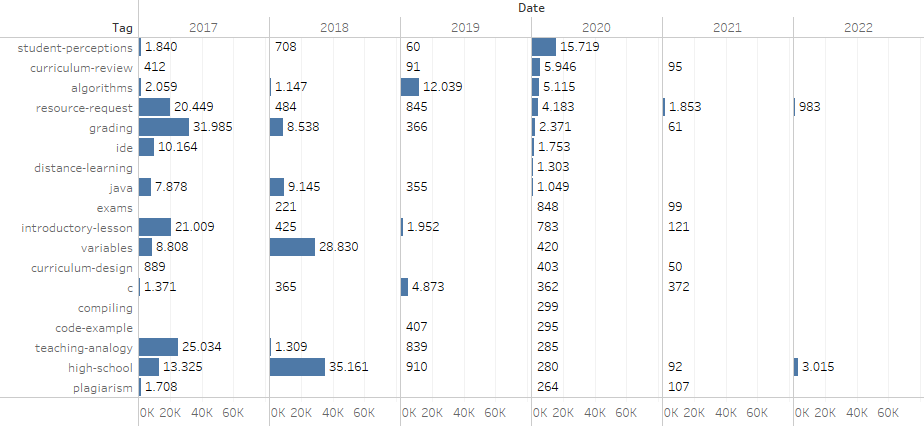
\includegraphics[width=\textwidth]{img/cse/tags_2020.png}
    \caption{ Distribución de etiquetas 2020 (Interfaz Tableau)}
    \label{figura:tags_2020}
\end{figure}


%%%%%%%%%%%%%%%%%%%%%%%%%%%%%%%%%%%%%%%%%%%%%%%%%%%%%%%%%%%%%%%%%%%%%%%
%\begin{figure}[ht]
%    \begin{minipage}[b]{0.45\linewidth}
%        \centering
%        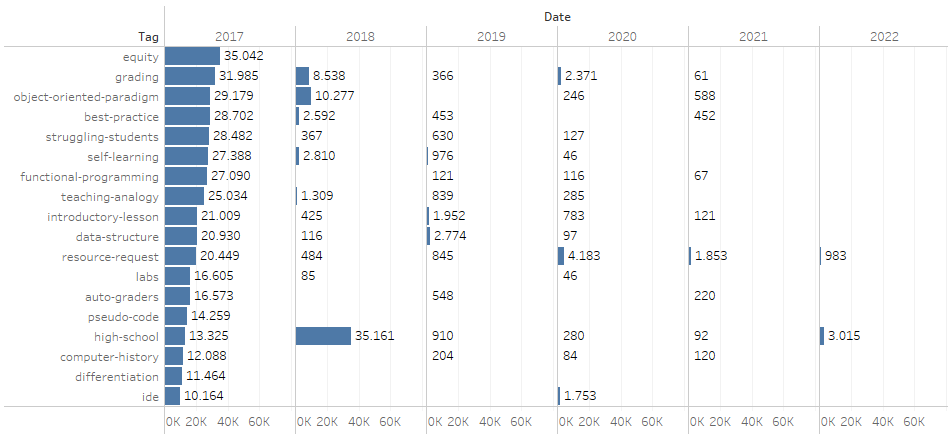
\includegraphics[width=\textwidth]{img/cse/tags_2017.png}
%        \end{minipage}
%    \hspace{0.5cm}
%    \begin{minipage}[b]{0.45\linewidth}
%       \centering
%        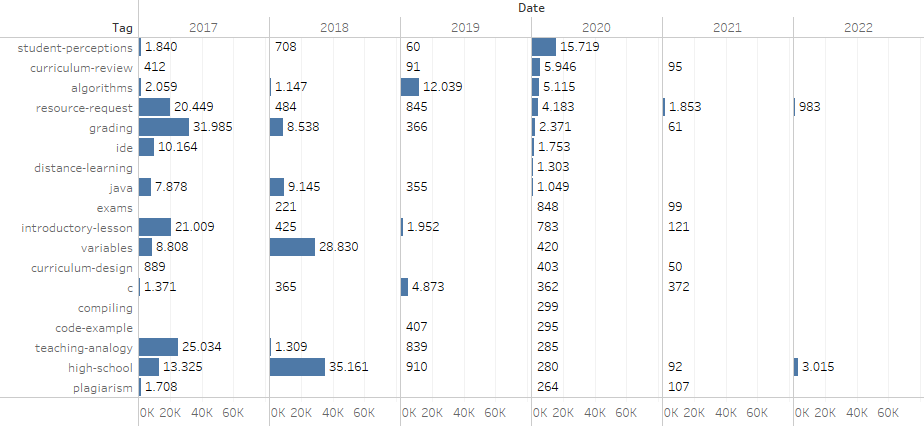
\includegraphics[width=\textwidth]{img/cse/tags_2020.png}
%    \end{minipage}
%    \caption{ Distribución de etiquetas diferenciando periodo temporal (Interfaz Tableau)}
%    \label{fig:tags_2017-2020}
%\end{figure}
%%%%%%%%%%%%%%%%%%%%%%%%%%%%%%%%%%%%%%%%%%%%%%%%%%%%%%%%%%%%%%%%%%%%%%


%
%



\subsection{Badges}

Lo primero a tratar es ¿qué son las \emph{bagdes}? Se trata de las insignias que se otorgan a los usuarios para dar reconocimiento a las contribuciones en la comunidad. 
Existen tres rangos de insignias: bronce, plata y oro. Las primeras son fáciles de obtener, suelen otorgarse a aquellos usuarios que enseñan a usar el sistema. Las segundas son aquellas que se obtienen por realizar publicaciones en la comunidad o realizar mejoras del sitio. Y, por último, las de oro, que representan una gran dedicación sobre la comunidad. 

Ahora que sabemos que son las insignias, otra medida para ver la evolución que presenta una comunidad o su tendencia es contabilizar esas insignias a lo largo del tiempo. Como es habitual, en los inicios de una comunidad la cantidad de preguntas y respuestas es mayor, y así hemos estado viéndolo en las diferentes representaciones. En este caso ocurre lo mismo, como se ha indicado, las insignias de bronce (clase 3) se obtienen por el uso del sistema o por generar preguntas. Por tanto durante el primer año se otorgan la mayor cantidad de insignias de bronce y va disminuyendo en los siguientes años. Las insignias de plata (clase 2) y oro (clase 1) al ser más complicadas de conseguir, se mantienen con poca oscilación en el tiempo. 

En la gráfica \ref{figura:badges} si que observamos un dato relevante, en torno al año 2021. Vemos que existe un incremento de insignias de bronce. Lo habitual es que fueran descendiendo como se observa en los años previos. Como hemos indicado \emph{cseducators} es una comunidad para profesionales de la educación, durante los años 2020 y 2021, la educación ha tenido que adaptarse y trabajar de manera online, por lo que puede que esta situación implique un uso mayor de la comunidad y por ello se vuelva a ver el incremento de insignias dentro de la comunidad.

\begin{figure}[ht]
    \centering
    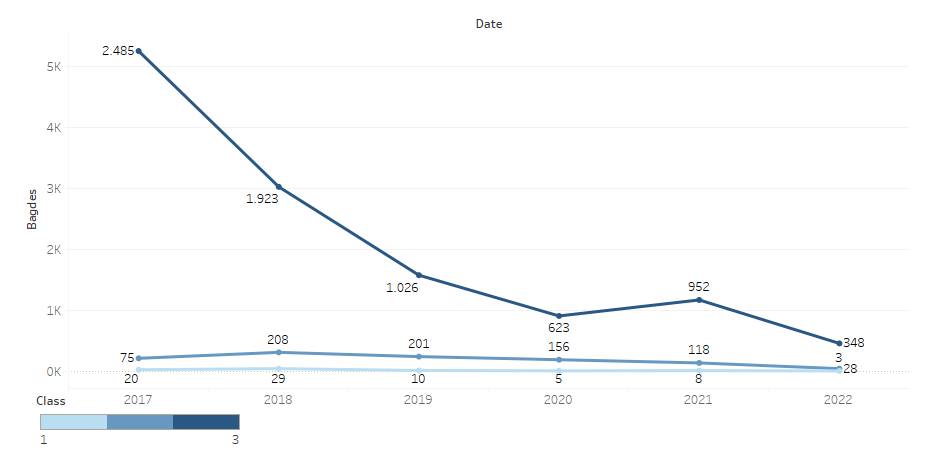
\includegraphics[width=\textwidth]{img/cse/badges.png}
    \caption{Panel: Distribución badges (Interfaz: Tableau)}
    \label{figura:badges}
\end{figure}


En la tabla \ref{tab:top_5_tags_cse} se muestran las insignias que más veces han sido otorgadas a los usuarios a lo largo del tiempo. 

\begin{table}[ht]
    \begin{center}
        \begin{tabular}{ c  l  l  }
        \hline
          \textbf{Class} & \textbf{Badge} & \textbf{Total} \\ \hline
            \multirow{5}{*}{Gold} & Famous Question & 36 \\ 
            & Fanatic & 33  \\ 
            & Great Answer & 7 \\
            & Populist & 7 \\ 
            & Great Question & 4 \\
            \hline
            \multirow{5}{*}{Silver} & Yearling & 621 \\ 
            & Good Answer & 113  \\ 
            & Notable Question & 124 \\
            & Good Question & 62 \\
            & Enthusiast & 58 \\ 
            \hline
            \multirow{5}{*}{Bronze} & Autobiographer & 4819 \\ 
            & Supporter & 2811 \\
            & Teacher & 909 \\ 
            & Informed & 649 \\ 
            & Editor & 556 \\
        \end{tabular}
        \caption{Insignias más populares CS Educators}
        \label{tab:top_5_tags_cse}
    \end{center}
\end{table}

\clearpage

\section{Experimento Tex}
\label{chap:exper_stack}

Al igual que en el dataset anterior crearemos la base de datos (\emph{tex}) en MySQL que utilizaremos en este experimento. Lanzaremos el script \texttt{load\_into\_pg.py} que descarga los ficheros, parsea los datos y los carga sobre la base creada.

Con el dataset extraído de Stack Exchange comentado, analizaremos nuevamente el comportamiento de las herramientas y analizaremos la comunidad en base a estos datos. 


\subsection{Usuarios}
En esta sección trabajaremos con los datos de la tabla \emph{users}, obteniendo los datos de usuarios existentes en la plataforma a lo largo del tiempo. Esta comunidad fue creada en 2010, por lo que los primeros usuarios son de esa fecha. A partir de ese momento, el número de usuarios se ve incrementado hasta la fecha actual. 

Representamos el total de usuarios existentes, como podemos observar en la gráfica \ref{figura:total_users_tex}, y a continuación mostramos la evolución y el crecimiento que ha presentado la plataforma con el paso del tiempo. 

Los datos tienen una fecha de extracción del 6 de junio de 2022, hasta este día podemos ver que hay un total de 223506 usuarios. 

\begin{figure}[ht]
    \centering
    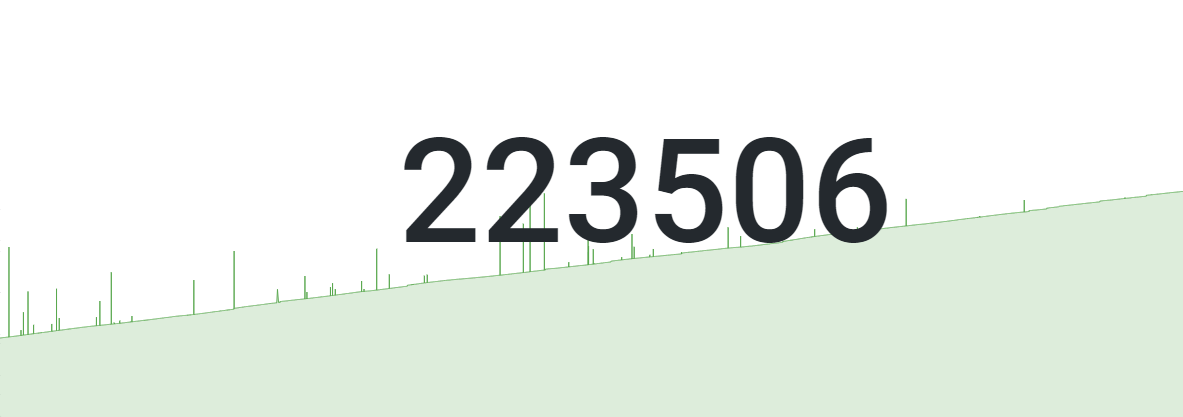
\includegraphics[width=0.5\textwidth]{img/tex/Total_usuarios_tex.png}
    \caption{Panel: Total de usuarios (Interfaz: Grafana)}
    \label{figura:total_users_tex}
\end{figure}


Al igual que en experimento anterior, este dato total aporta una visión general pero no observamos la evolución de la plataforma. Para ello, se procede a generar otras visualizaciones que desglosan estos datos por años, observando la evolución total de la comunidad.

\begin{figure}[ht]
    \centering
    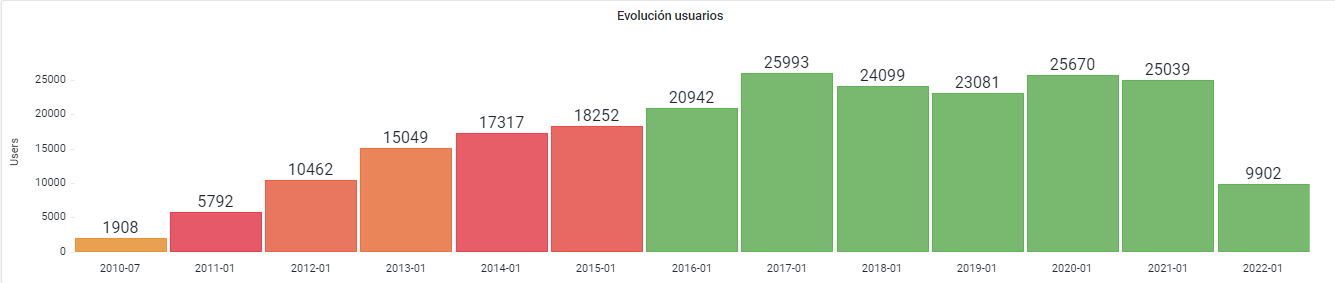
\includegraphics[width=0.6\textwidth]{img/tex/evolucion_usuarios_tex.png}
    \caption{Panel: Evolución anual de usuarios (Interfaz: Grafana)}
    \label{figura:evo_users_tex}
\end{figure}

Como se puede ver en la figura \ref{figura:evo_users_tex}, esta comunidad tiene un crecimiento lineal. Al crearse la comunidad el número de usuarios registrados es reducido, se van duplicando el número de usuarios en los primeros años llegando a registrarse casi 20 mil usuarios anualmente en los primeros 5 años de la plataforma. Tras ese primer momento, se observa que desde 2017 el registro de usuarios es más estable con una variación de centenas de usuarios.

Con esta visión más general podemos ver que hay dos grandes periodos, uno desde la creación de esta hasta 2015 que sería el periodo de mayor crecimiento, y otro, desde 2017 hasta la actualidad que nos muestra la estabilidad de la plataforma. Para mostrarlo, por cada año agruparemos los datos en trimestres. 

Si vemos detenidamente la gráfica \ref{figura:evo_users_trim_tex}, que corresponde con los datos desde 2010 hasta 2016, presenta una tendencia exponencial creciente. Podemos ver que habitualmente la mayor cantidad de registros se presenta de forma habitual en el cuarto trimestre. En la gráfica \ref{figura:evo_users_trim_tex_2} vemos el siguiente periodo, desde 2017 hasta la actualidad. En este plazo el registro es más estable. En ambas imágenes destaca que el tercer trimestre es un periodo de menor registro en la comunidad. 

\begin{figure}[ht]
    \centering
    \includegraphics[width=0.75\textwidth]{img/tex/evolucion_usuarios_años_tex_1.png}
    \caption{Panel: Evolución trimestral de usuarios (Interfaz: Tableau)}
    \label{figura:evo_users_trim_tex}
\end{figure}

\begin{figure}[ht]
    \centering
    \includegraphics[width=0.75\textwidth]{img/tex/evolucion_usuarios_años_tex_2.png}
    \caption{Panel: Evolución trimestral de usuarios (Interfaz: Tableau)}
    \label{figura:evo_users_trim_tex_2}
\end{figure}

Con los datos extraídos y analizados en la herramienta de Tableau, podemos realizar un pronóstico de crecimiento de la plataforma siguiendo la tendencia existente. Esta información se muestra en la gráfica \ref{figura:tendencia_tex}, según este modelo el número de nuevos usuarios seguirá descendiendo.

\begin{figure}[ht]
    \centering
    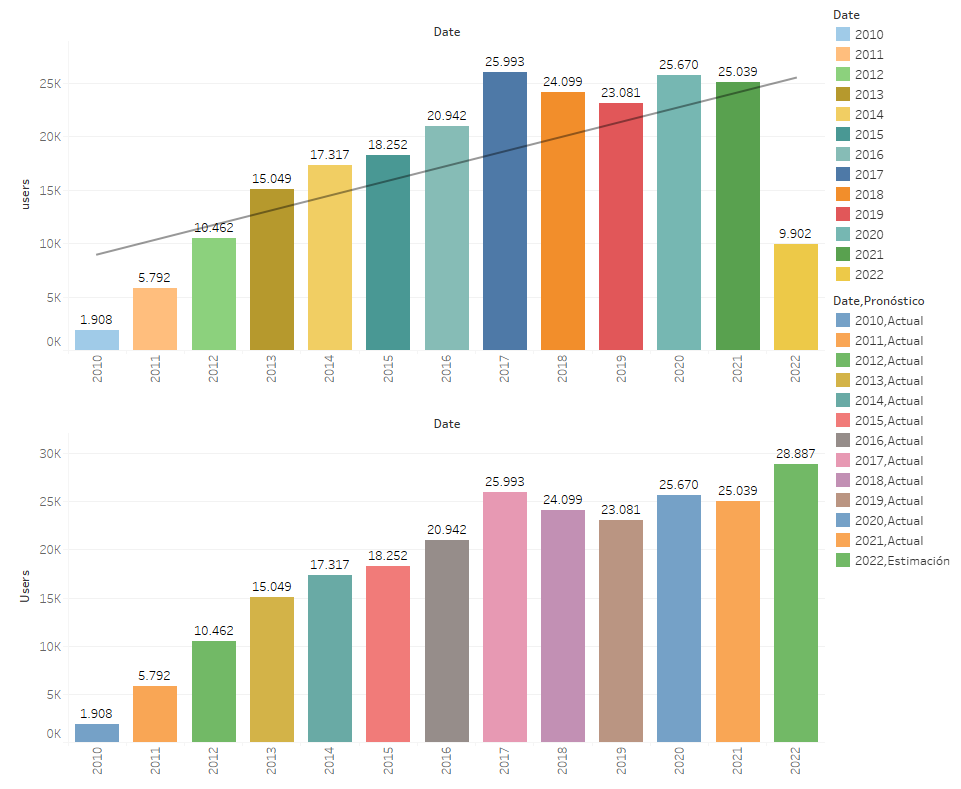
\includegraphics[width=0.6\textwidth]{img/tex/Tendencia_pronostico_TEX.png}
    \caption{Panel: Tendencia y pronóstico 2022 TEX (Interfaz: Tableau)}
    \label{figura:tendencia_tex}
\end{figure}

Una de las opciones de visualización que nos ofrecen las herramientas utilizadas en este trabajo, es la visualización de los datos en mapas geográficos. La localización es un campo existente entre la información de los usuarios. Si observamos la figura \ref{figura:MAP_users_tex} vemos los países presentan mayor cantidad de usuarios. No se encuentran disponibles todos los datos, esto se debe a que la localización es un campo de texto libre, por tanto, no sigue un patrón determinado, existen múltiples valores que no son ubicaciones reales (IPs, "Earth", "MyHome",etc) o diferentes nombres para una misma ubicación (España, Espagna, Spain, (E)spain, etc.) por tanto, se tiene que realizar un filtrado o unificación de esos datos y excluir todos los valores que no contienen una ubicación real. Así mismo, muchos usuarios no incluyen el dato de localización, siendo este un campo a \emph{NULL}. 

\begin{figure}[ht]
    \centering
    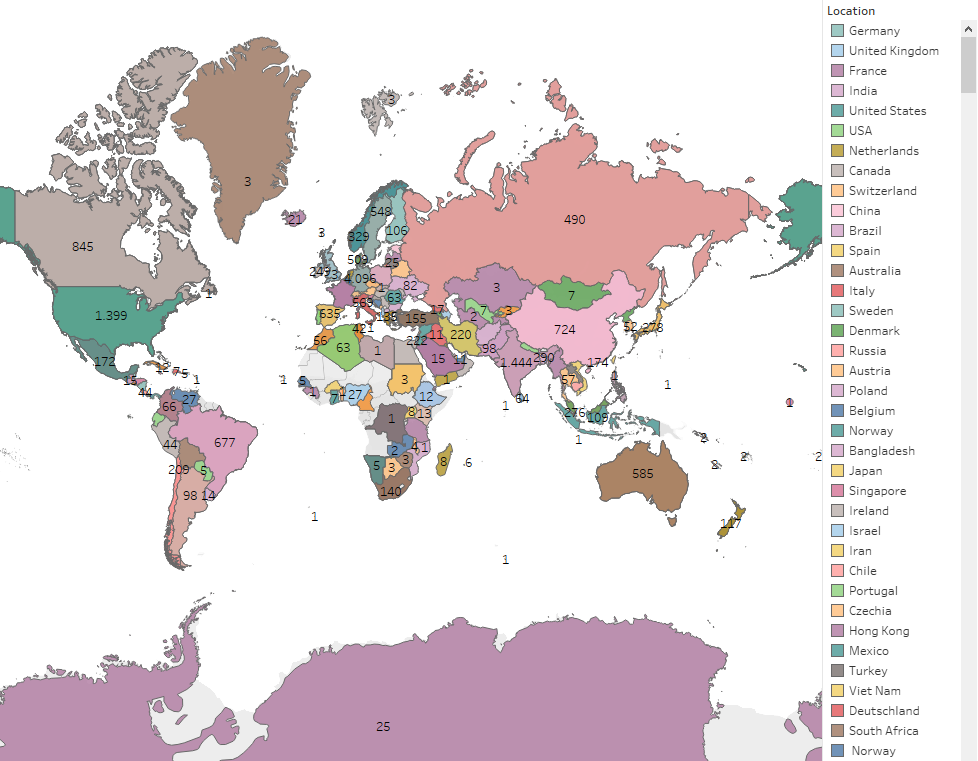
\includegraphics[width=0.75\textwidth]{img/tex/Maps_tex.png}
    \caption{Panel: Localización de usuarios Tex (Interfaz: Tableau)}
    \label{figura:MAP_users_tex}
\end{figure}

\clearpage
%Las visualizaciones se realizan en ambas herramientas, el procesado de estos varía según la herramienta, pero se muestran siguiendo los mismos criterios.


\subsection{Publicaciones}

En esta sección observamos las publicaciones realizadas, dentro de las comunidades de pregunta/respuesta las publicaciones realizadas nos permiten ver la evolución de la plataforma en el tiempo. 

En la figura \ref{figura:evo_post_anual_tex} se muestra que durante los primeros dos años la comunidad presenta pocas entradas de preguntas y/o respuestas, aumentando de manera relevante en los siguientes años hasta la actualidad. Tex es una comunidad sobre sistemas de tipografía usadas principalmente en documentación científica y matemática. El aumento de actividad puede estar asociado al uso de estas tipografías para documentos, informes, libros, etc. 

\begin{figure}[ht]
   \centering
    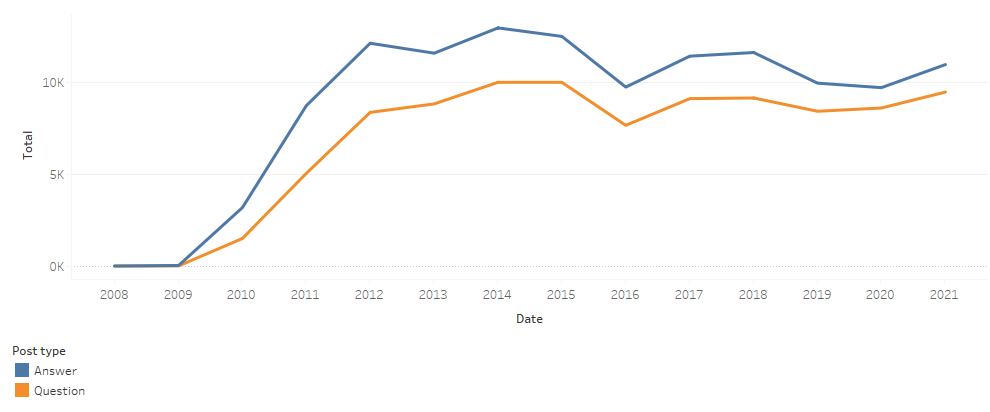
\includegraphics[width=0.8\textwidth]{img/tex/evo_posts_anual_tex.png}
    \caption{Panel: Evolución pregunta/respuesta (Interfaz: Tableau)}
    \label{figura:evo_post_anual_tex}
\end{figure}

Dentro de la publicación se pueden obtener datos adicionales relacionados. Uno de estos valores sería la puntuación, que contabiliza el número de votos positivos menos el número de votos negativos, obteniendo así el valor que presenta la publicación. 

También podemos ver el indicador de favoritos, que contabiliza el número de veces que una publicación ha sido guardada por los usuarios de la plataforma. En la tabla \ref{table:top_5_tex} podemos ver un ejemplo del top 5 de los \emph{posts} con mayor número de favoritos de la comunidad con el \emph{link} al post y la puntuación otorgada por los usuarios y su título. 
\begin{table}[ht]
\centering
    \begin{tabular}{@{} p{2cm} p{6cm} p{1cm} p{2cm} @{}}
        \hline
        Post link & Title & Score & Favorite \\
        \hline
        4425 & Is there a way to have coloured hyperref hyperlinks in the PDF \ldots & 94 & 46 \\
        2547 & Margin Figures/Captions & 26 & 12 \\
        2897 & Where to place custom beamer themes & 30 & 12 \\
        3881 & Formatting a paragraph to look like a section & 21 & 5 \\
        5023 & Aligning an enumeration item to the top of a tikzpicture & 17 & 4 \\ 
        \hline
    \end{tabular}
\caption{Top 5 Publicaciones favoritas de la comunidad Tex}
\label{table:top_5_tex}
\end{table}

%******************************
%Unanswered Questions
%questions with no upvoted or accepted answers
%Meter la info de publicaciones sin respuesta.
%******************************



\subsection{Tags}
Las etiquetas identifican la conexión entre las preguntas publicadas y los expertos. También suelen usarse para identificar preguntas interesantes o relevantes para los usuarios de la comunidad. 

Las bases son semejantes en todas las comunidades, existiendo límites por cada pregunta, creación de nuevas etiquetas, reemplazo de espacios por guiones \ldots Las etiquetas de la publicación también sirven para realizar búsquedas más rápidas dentro de la comunidad. Por tanto, la relación existente entre las etiquetas y el número de visualizaciones de las publicaciones las contienen es una información a revisar en cualquier plataforma de pregunta/respuesta.

En la figura \ref{figura:top10_tags_tex} vemos el \textbf{top 10} de las etiquetas más populares de \emph{Tex} de forma individual durante todo el periodo activo de la plataforma. Se ha extraído la información de cada etiqueta utilizada, no del uso habitual que pueda observarse en las publicaciones. Vemos que entre las etiquetas que aparecen más veces se encuentra \emph{tikz-pgf} o \emph{pgfplots}, ambas están asociadas a la visualización y creación de gráficos científicos/ técnicos. 

Por otro lado, en la imagen \ref{figura:evo_tags_tex} se ve representado el \textbf{top 10} de las etiquetas más usadas de forma conjunta durante todo el periodo activo y el número de visualizaciones que obtienen las publicaciones en las que se encuentran estas \emph{tags}. 

\begin{figure}[ht]
    \centering
    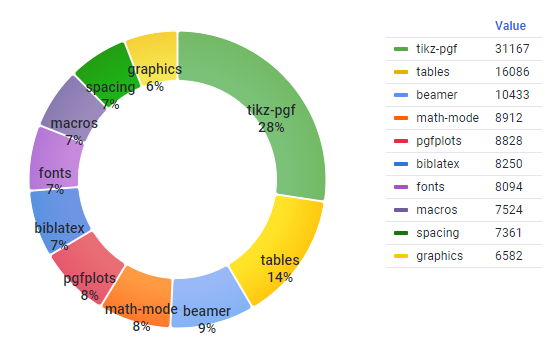
\includegraphics[width=0.6\textwidth]{img/tex/tags_evo_tex.png}
    \caption{Panel: Top 10 etiquetas (Interfaz: Grafana)}
    \label{figura:top10_tags_tex}
\end{figure}

\begin{figure}[ht]
    \centering
    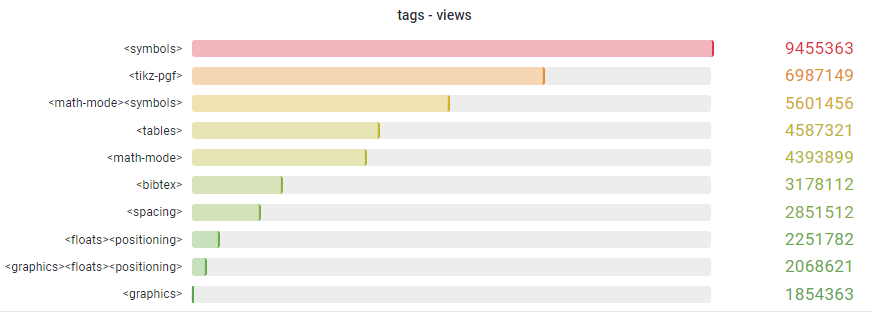
\includegraphics[width=0.6\textwidth]{img/tex/evo_tags_tex.png}
    \caption{Panel: Top 10 etiquetas conjuntas más visualizadas (Interfaz: Grafana)}
    \label{figura:evo_tags_tex}
\end{figure}

Podemos desglosar y comparar estos datos en el mismo mes, pero de diferente periodo. Hemos decidido tomar los valores del mes de abril, ya que es un mes de alta actividad en la plataforma, y veremos las diferencias entre el \textbf{top 10} de \emph{tags} más usadas entre el año 2016 y el actual (2022). En la imagen \ref{figura:comp_tags_tex} observamos que apenas tenemos un uso semejante, únicamente observamos que se usa la etiqueta \emph{graphics} en ambos periodos.

En el año 2016 las etiquetas más utilizadas hacen referencia a bibliotecas, formateo de texto, diseño\ldots mientras que en la actualidad se hace uso de etiquetas sobre los tipos de gráficas, fuentes de texto \ldots En otras palabras, en los primeros años se publica en la comunidad sobre la información general, es decir, cómo aplicar los diferentes sistemas tipográficos o cómo dar forma a los textos. Mientras que en la actualidad se observa mediante las etiquetas que estos sistemas de tipografía son más utilizados entre la población, ya que entre las \emph{tags} más usadas se alude a diferentes formas de visualización más especificas.

\begin{figure}[ht]
    \centering
    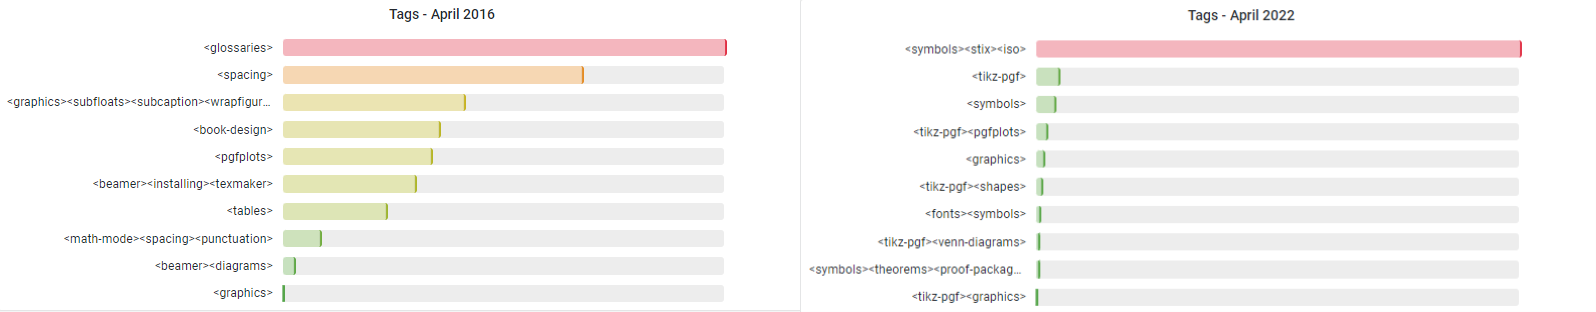
\includegraphics[width=\textwidth]{img/tex/Compare_tags_april_tex.png}
    \caption{Comparación de etiquetas Abril 2016 - Abril 2022 (Interfaz: Grafana)}
    \label{figura:comp_tags_tex}
\end{figure}



\subsection{Badges}

Como se ha identificado en el experimento anterior las \emph{bagdes}, son las insignias que se otorgan a los usuarios dando reconocimiento a las distintas contribuciones dentro de la comunidad. 
Se basa también en los mismos tres rangos de insignias: bronce, plata y oro. Las primeras más sencillas de obtener, las segundas que se obtienen por realizar publicaciones o mejoras del sitio. Y, por último, las de oro, que representan una gran dedicación en la comunidad. 

En la gráfica \ref{figura:badges_tex} vemos la evolución de las insignias diferenciadas por cada clase. Esta plataforma, como indicamos al principio de la sección, contiene aproximadamente 223 mil usuarios y las insignias que se han otorgado a lo largo del tiempo acreditan que se trata de una comunidad activa con gran cantidad de contribuciones por parte de los usuarios. 

\begin{figure}[ht]
    \centering
    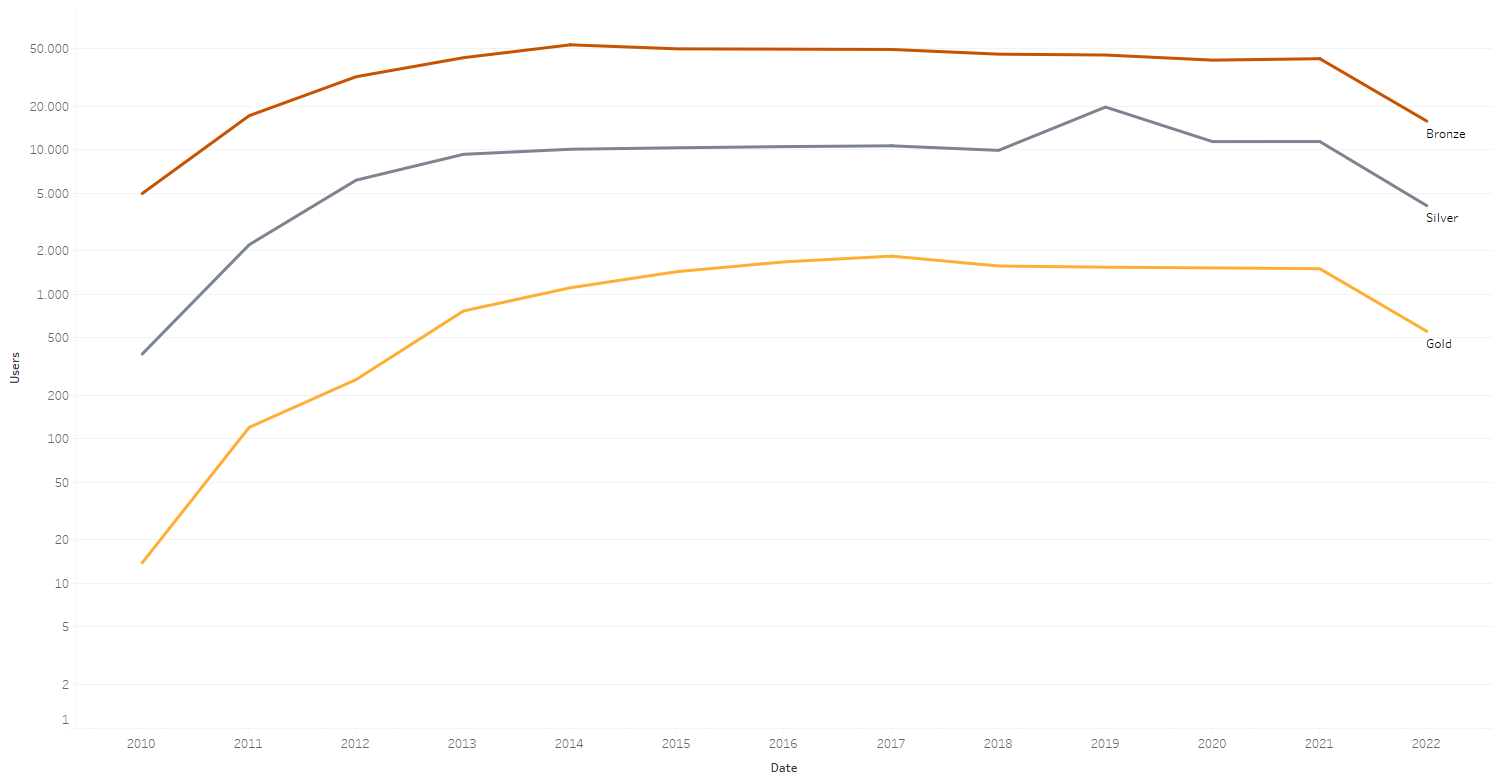
\includegraphics[width=0.8\textwidth]{img/tex/badges_tex.png}
    \caption{Panel: Distribución badges asociadas a Tags (Interfaz: Grafana)}
    \label{figura:badges_tex}
\end{figure}


Dentro de estas clases de insignias podemos particularizarlas en dos grupos: las asociadas a \emph{tags} y otras asociadas a los logros obtenidos. En el gráfico \ref{figura:badges_tag_tex_dist} observamos el porcentaje de asignación de las insignias relacionadas con las etiquetas divididas por cada una de las clases. Centrándonos en esos datos y realizando desglose de esos datos, podemos obtener el listado (top 10) de estas etiquetas como se muestra en la imagen \ref{figura:badges_tags_data_tex}. Vemos que, al igual que en las tags, una de las insignias más recurrentes es \emph{tikz-pgf}, además vemos que la mayoría de ellas se repiten, ya que es habitual su uso dentro de esta comunidad.

\begin{figure}[ht]
    \centering
    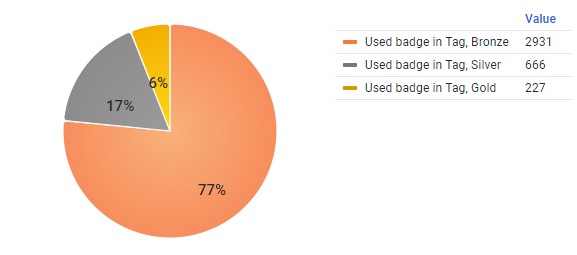
\includegraphics[width=0.6\textwidth]{img/tex/Badges_tag_tex_dist.png}
    \caption{Porcentaje de insignias asociadas a etiquetas (Interfaz: Grafana)}
    \label{figura:badges_tag_tex_dist}
\end{figure}

\begin{figure}[ht]
    \centering
    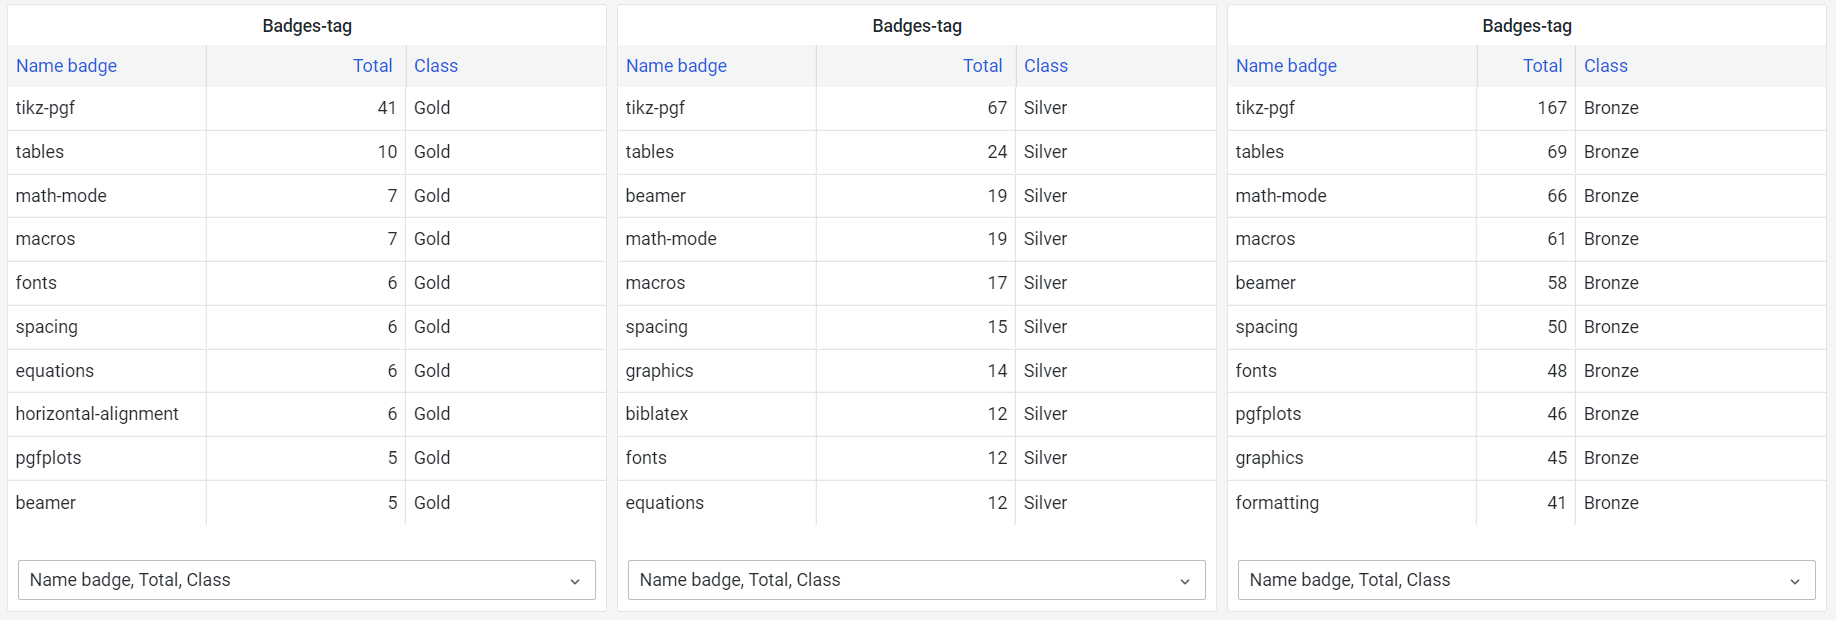
\includegraphics[width=0.6\textwidth]{img/tex/Badges_tag_tex_data.png}
    \caption{Comparación de etiquetas Abril 2016 - Abril 2022 (Interfaz: Grafana)}
    \label{figura:badges_tags_data_tex}
\end{figure}

Por otra parte, tenemos las insignias que se entregan a los usuarios por los logros realizados en la comunidad. En una comunidad de pregunta/respuesta la mayor parte de las insignias que se conceden son de este tipo, sin estar asociadas a las etiquetas. En este caso, como se puede ver en el gráfico \ref{figura:badges_tex_dist}, las insignias de tipo oro son inferiores a las que se observaban en los datos anteriores. Estas etiquetas son más complicadas de obtener ya que pueden estar asociados a realizar pregunta o respuestas, como puede ser obtener puntos  o marcas de favorito, de moderación por revisar tareas o marcar publicaciones, o simplemente por participar en la comunidad como, por ejemplo, visitar de manera consecutiva la plataforma, etc. 

\begin{figure}[ht]
    \centering
    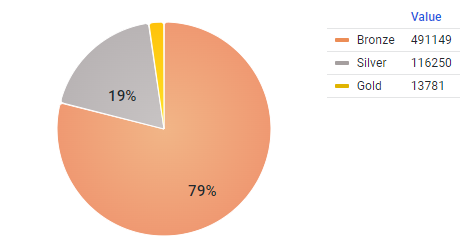
\includegraphics[width=0.6\textwidth]{img/tex/Badges_tex_dist.png}
    \caption{Porcentaje de insignias asociadas a etiquetas (Interfaz: Grafana)}
    \label{figura:badges_tex_dist}
\end{figure}

En la tabla \ref{tab:top_5_tags_tex} se muestra el \textbf{Top 5} por cada clase, de manera que están representadas aquellas que más veces han sido otorgadas a los usuarios a lo largo del tiempo. 

\begin{table}[ht]
    \begin{center}
        \begin{tabular}{ c  l  l  }
        \hline
          \textbf{Class} & \textbf{Badge} & \textbf{Total} \\ \hline
            \multirow{5}{*}{Gold} & Famous Question & 10501 \\ 
            & Great Answer & 816 \\
            & Great Question & 636 \\
            & Fanatic & 616  \\ 
            & Electorate & 267 \\ 
            \hline
            \multirow{5}{*}{Silver} & Yearling & 38222 \\ 
            & Notable Question & 34061 \\
            & Enlightened & 13933 \\
            & Good Answer & 7662  \\ 
            & Necromancer & 7281 \\ 
            \hline
            \multirow{5}{*}{Bronze} & Popular Question & 69965 \\ 
            & Student & 66778 \\
            & Supporter & 57423 \\
            & Autobiographer & 54950 \\ 
            & Scholar & 43479 \\ 
        \end{tabular}
        \caption{Insignias más populares - TEX}
        \label{tab:top_5_tags_tex}
    \end{center}
\end{table}


Las \emph{badges} nos muestran información con la que podemos obtener \emph{rankings} semanales, mensuales, etc. de los usuarios que han obtenido más insignias tanto de manera global como por cada tipo. 
En la imagen \ref{figura:badges_tex_top} podemos ver los usuarios con mayor número de \emph{badges} clasificados por la reputación que presentan dentro de la plataforma. Y en la imagen \ref{figura:badges_tex_class_top} veremos esta clasificación separada por cada tipo de clase y la reputación del usuario.
Se puede observar que la reputación y las insignias de los usuarios están relacionadas, ya que aquellos con más reputación, presentan mayor número de insignias de cada tipo. 

\begin{figure}[ht]
    \centering
    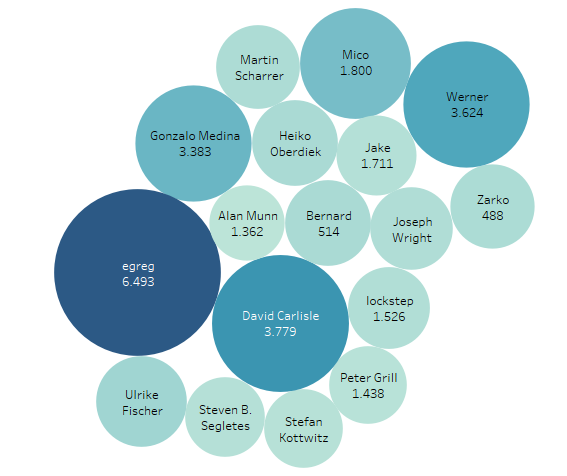
\includegraphics[width=0.8\textwidth]{img/tex/Popular_users_badges_tex.png}
    \caption{Usuarios con más insignias (Interfaz: Tableau)}
    \label{figura:badges_tex_top}
\end{figure}


\begin{figure}[ht]
 \centering
  \subfloat[Gold]{
   \label{f:oro}
    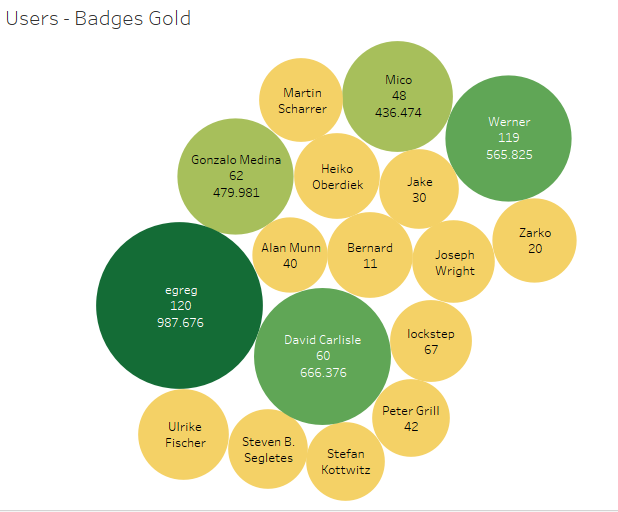
\includegraphics[width=0.3\textwidth]{img/tex/Popular_users_badges_tex_1.png}}
  \subfloat[Silver]{
   \label{f:plata}
    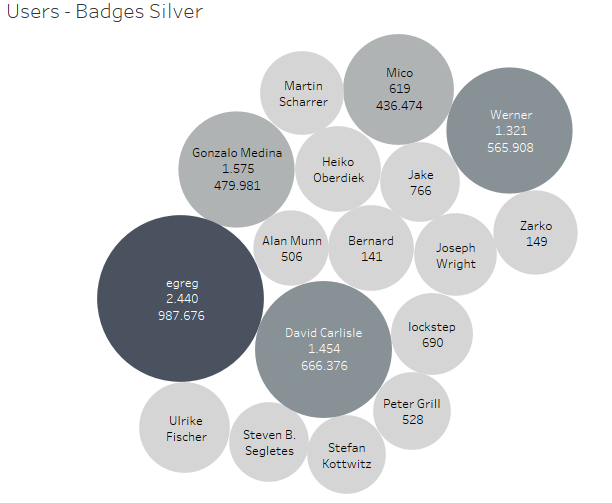
\includegraphics[width=0.3\textwidth]{img/tex/Popular_users_badges_tex_2.png}}
  \subfloat[Bronze]{
   \label{f:bronce}
    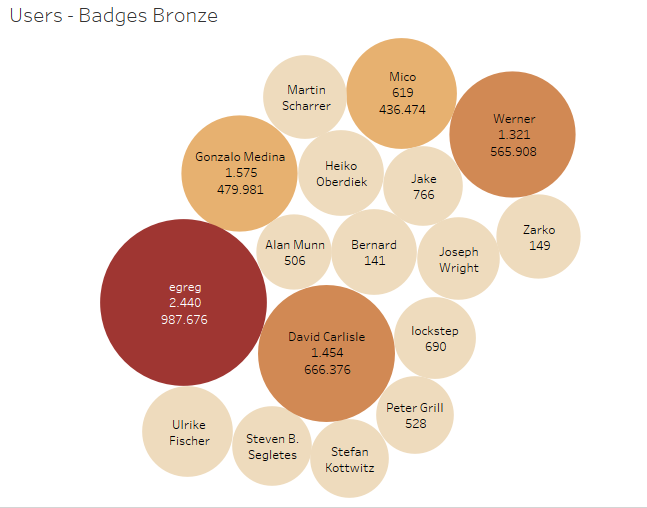
\includegraphics[width=0.3\textwidth]{img/tex/Popular_users_badges_tex_3.png}}
 \caption{Usuarios con más insignias por clase (Interfaz: Tableau)}
 \label{figura:badges_tex_class_top}
\end{figure}

\clearpage 

\section{Comparativa de comunidades}
\label{chap:compare_community}

Durante este capítulo hemos desarrollado diferentes visualizaciones que nos permiten conocer ligeramente cada comunidad. En el caso del dataset de Computer Science Educators hemos comprobado que se trata de una comunidad de una pequeña cantidad de usuarios y poca actividad. La mayoría de los usuarios, publicaciones y contribuciones, tanto de preguntas como respuestas, fueron registrados en los primeros años y van reduciéndose en el tiempo. En cambio, en el segundo dataset, correspondiente con la comunidad de Tex, hemos notado que el registro presenta una tendencia creciente tanto a nivel de usuarios como publicaciones. Esto nos indica que se trata de una plataforma activa y que aun continúa en crecimiento. El número de usuarios hemos visto que aumenta por cada periodo y se pronostica que seguirá creciendo según la tendencia actual. Este mismo comportamiento se produce en las publicaciones.

Tomando como referencia las etiquetas existentes, otro de los factores utilizados para las visualizaciones, hemos observado que, en la comunidad de CS Educators, principalmente se usan etiquetas conjuntas que hacen que las búsquedas y las publicaciones estén bastante relacionadas. En el caso de las insignias, podemos identificar que no existen grandes contribuciones o logros de manera habitual. El usuario que tiene más reputación en la plataforma tiene 1293 insignias de las tres clases.
En cambio, en la comunidad de Tex hemos comprobado que existe diversidad de etiquetas, que son utilizadas tanto de manera conjunta como de forma individual y además, estas etiquetas están presentes en los usuarios cuando se obtienen sus insignias. Aparte, de manera individual, por cada usuario hemos podido ver que se asignan múltiples insignias y podríamos realizar diversos \emph{rankings} ya que se otorgan diariamente incrementando la reputación de los usuarios. 

Se ha trabajado con otro de los campos que ofrece el registro de usuarios, la localización. En el primer dataset, teníamos en torno a dos mil datos de localización, el filtrado es relativamente sencillo aunque siga teniendo que realizarse un preprocesado debido a los múltiples valores existentes sobre un mismo lugar.  En el dataset de Tex, al tener un mayor número de usuarios, disponemos de más información y al tener más información, el filtrado de datos es más complicado. Por esto mismo, aunque se haya podido visualizar sobre la interfaz de Tableau, los datos mostrados en el mapa no son del todo fiables, requiere de mayor preprocesado. 


\cleardoublepage

%%%%%%%%%%%%%%%%%%%%%%%%%%%%%%%%%%%%%%%%%%%%%%%%%%%%%%%%%%%%%%%%%%%%%%%%%%%%%%%%
%%%%%%%%%%%%%%%%%%%%%%%%%%%%%%%%%%%%%%%%%%%%%%%%%%%%%%%%%%%%%%%%%%%%%%%%%%%%%%%%
% CONCLUSIONES %
%%%%%%%%%%%%%%%%%%%%%%%%%%%%%%%%%%%%%%%%%%%%%%%%%%%%%%%%%%%%%%%%%%%%%%%%%%%%%%%%


\chapter{Conclusiones y trabajos futuros}
\label{chap:conclusiones}
En este capítulo se expondrán las conclusiones finales del proyecto y los objetivos alcanzados.

\section{Consecución de objetivos}
\label{sec:consecucion-objetivos}

En este proyecto indicamos dos objetivos principales. Por un lado, se ha conseguido analizar el conjunto de datos extraídos de la plataforma de Stack Exchange, para ello definimos el alcance del proyecto, se realizó la recolección, parseado e inserción de los datos, mediante el desarrollo de un programa que nos permite realizar estos pasos. Y por último, la visualización de cada base de datos en las herramientas software, centrándonos en dos de las herramientas más utilizadas en la actualidad como son Tableau y Grafana para estudiar bases de datos temporales. 

Por otra parte, de manera más específica nos propusimos también evaluar estas herramientas en base una serie criterios de comparación. 

Lo primero que se observó al realizar el estudio de las herramientas, es la diferencia entre Tableau y Grafana. La primera, realmente es un conjunto de herramientas de inteligencia de negocios que presenta un licenciamiento y un coste asociado dependiendo del tipo de usuarios y las funcionalidades que se requieran. En nuestro caso, hemos realizado este proyecto mediante una prueba gratuita, que se ofrece para conocer las herramientas. En cambio Grafana, aunque tiene una versión comercial, es un software de código libre por tanto no requiere una licencia ni coste adicional. 

Tras realizar el análisis de los datos hemos podido identificar que Tableau presenta una interfaz de usuario mucho más sencilla y no es necesario conocer el flujo completo de datos para poder realizar un análisis simple. Además, el preprocesado se puede optimizar creando flujos previos mediante la herramienta Tableau Prep y ser reutilizados en otros datasets. En cambio, Grafana, presenta una interfaz menos amigable y basada en \gls{plugin}, es recomendable tener un mayor conocimiento del conjunto de datos para poder realizar las mismas gráficas.
De cara al tamaño de las muestras ambas herramientas son compatibles con cualquier magnitud de datos y ofrecen prácticamente las mismas opciones de visualización. 

Podemos destacar el problema encontrado en el gráfico en forma de mapas, es significativo con nuestro conjunto de datos ya que este valor de campo es texto libre. Grafana permite visualizar los datos siempre que se representen en forma de función geográfica (latitud y longitud), para ello requeríamos de un reprocesado de nuestros datos, por lo que por tiempos no ha sido posible aplicar esta visualización en esta herramienta. Mientras que Tableau geocodifica las localizaciones de manera directa si son países, ubicaciones, códigos postales. Por tanto en nuestro caso, después de un pequeño preprocesado para agrupar los datos, se han podido mostrar sin problemas.

Principalmente cada herramienta esta diseñada para representar un conjunto de datos específicos, por ejemplo Grafana está más enfocado en ofrecer monitorización y alertas de datos en real-time y Tableau, en cambio, esta más orientado en comparar datos ya que presta más atención a la inteligencia empresarial.


%\begin{minted}{bash}
%  aspell --lang=es_ES -c memoria.tex
%\end{minted}

\section{Aplicación de lo aprendido}
\label{sec:aplicacion}

En el desarrollo de este proyecto, han sido de utilidad los conocimientos adquiridos en varias asignaturas. Estas son:

\begin{itemize}
  \item \textbf{Sistemas Operativos}: Primer contacto con la programación, necesaria para tener una buena base tanto en las asignaturas de la carrera como en mi actual vida laboral. 
  \item \textbf{Servicios y Aplicaciones Telemáticas}: donde comencé a usar el lenguaje de programación \emph{Python}, parte fundamental del desarrollo de este trabajo y conocer \emph{Git} que es el sistema de control de versiones distribuido utilizado para el almacenamiento del proyecto. 
  \item \textbf{Ingeniería de sistemas de Información}: supuso el primer contacto con las bases de datos relacionales y el lenguaje SQL.
  \item \textbf{Ingeniería de Sistemas Telemáticos}: donde senté las bases del paradigma de la programación orientada a objetos (OOP), necesarios para la creación del programa de procesado ya que \emph{Python} es un lenguaje orientado a objetos.
\end{itemize}


\section{Lecciones aprendidas}
\label{sec:lecciones_aprendidas}

Durante el desarrollo de este Trabajo de Fin de Grado, se pueden destacar las siguientes lecciones aprendidas:

\begin{enumerate}
  \item Profundizar en datasets de distintas magnitudes, lo que me ha permitido ampliar los conocimientos aprendidos durante las asignaturas de la carrera.
  \item Incrementar mis habilidades de programación en \emph{Python} manejando estructuras XML y en el tratamiento de bases de datos MySQL.
  \item Conocer y aprender la programación en \LaTeX, ya que hasta la realización de esta memoria, no lo había utilizado.
  \item Ampliar el conocimiento en la visualización de datos y la importancia del procesamiento de datos para lograr obtener datos relevantes y poder interpretar los resultados de manera correcta. 
\end{enumerate}


\section{Trabajos futuros}
\label{sec:trabajos_futuros}
El posible desarrollo futuro de este proyecto requeriría, en primer lugar, de un preprocesado de datos mejorado, para evitar los problemas encontrados en la visualización de estos en las gráficas de geolocalización. 

También se puede ampliar la información existente los datasets, ya que contienen el esquema completo de estas comunidades contienen mucha información relacional que no se ha mostrado durante este proyecto y aportan datos útiles para conocer las comunidades.

Podría sería interesante poder comparar los resultados obtenidos con otras herramientas existentes como Splunk o introducir Graphite que permite, entre otras cosas, agregar funciones, combinar series temporales, modificar y/o añadir parámetros.

También sería interesante automatizar la descarga de los datos de forma que siempre se encontrasen actualizadas en las herramientas y tener un seguimiento real-time de las medidas más interesantes de las comunidades de pregunta y respuesta.

%%%%%%%%%%%%%%%%%%%%%%%%%%%%%%%%%%%%%%%%%%%%%%%%%%%%%%%%%%%%%%%%%%%%%%%%%%%%%%%%
%%%%%%%%%%%%%%%%%%%%%%%%%%%%%%%%%%%%%%%%%%%%%%%%%%%%%%%%%%%%%%%%%%%%%%%%%%%%%%%%
% GLOSARIO(S) %
%%%%%%%%%%%%%%%%%%%%%%%%%%%%%%%%%%%%%%%%%%%%%%%%%%%%%%%%%%%%%%%%%%%%%%%%%%%%%%%%
\glsaddall
\printglossary[type=\acronymtype]
\printglossary

%%%%%%%%%%%%%%%%%%%%%%%%%%%%%%%%%%%%%%%%%%%%%%%%%%%%%%%%%%%%%%%%%%%%%%%%%%%%%%%%
%%%%%%%%%%%%%%%%%%%%%%%%%%%%%%%%%%%%%%%%%%%%%%%%%%%%%%%%%%%%%%%%%%%%%%%%%%%%%%%%
% APÉNDICE(S) %
%%%%%%%%%%%%%%%%%%%%%%%%%%%%%%%%%%%%%%%%%%%%%%%%%%%%%%%%%%%%%%%%%%%%%%%%%%%%%%%%

%\cleardoublepage
%\appendix
%\chapter{Manual de usuario}
%\label{app:manual}


%%%%%%%%%%%%%%%%%%%%%%%%%%%%%%%%%%%%%%%%%%%%%%%%%%%%%%%%%%%%%%%%%%%%%%%%%%%%%%%%
%%%%%%%%%%%%%%%%%%%%%%%%%%%%%%%%%%%%%%%%%%%%%%%%%%%%%%%%%%%%%%%%%%%%%%%%%%%%%%%%
% BIBLIOGRAFIA %
%%%%%%%%%%%%%%%%%%%%%%%%%%%%%%%%%%%%%%%%%%%%%%%%%%%%%%%%%%%%%%%%%%%%%%%%%%%%%%%%

\cleardoublepage


% https://www.overleaf.com/learn/latex/Bibliography_management_with_biblatex
\raggedright\printbibliography[heading=bibintoc,title={Referencias}]

\end{document}
